% v1: November 2021
\documentclass[11pt]{article}
\pdfoutput=1
\usepackage{mathStyle}
%\usepackage{jhepmod}
\usepackage{fancyhdr}
\usepackage{amsmath,amssymb,amsthm,latexsym,bbm,calc,wasysym,mathtools,empheq, yfonts,upgreek}
\usepackage[english]{babel}
\usepackage{relsize}
\usepackage{graphicx}
\usepackage{upgreek}
\definecolor{rindou1}{rgb}{0.4431,0.2862,0.7960}
\definecolor{rindou2}{rgb}{0.078,0.1215,0.4392}
\definecolor{BrickRed}{rgb}{0.8, 0.25, 0.33}
\definecolor{mycolor}{rgb}{0.322, 0.565, 0.988}
\usepackage{esint} 
\pdfoutput=1
\usepackage[T1]{fontenc}
\usepackage{slashed}
\usepackage{verbatim} 
\usepackage{listings}
\usepackage{color}
\usepackage{datetime2}
\usepackage{lmodern}
\usepackage[x11names]{xcolor}
\usepackage{framed}
\colorlet{shadecolor}{LavenderBlush2} 
\colorlet{framecolor}{Red1}
\usepackage[framemethod=tikz]{mdframed}
\usepackage{xcolor}
\newmdenv[innerlinewidth=0.3pt, roundcorner=2pt,linecolor=mycolor,innerleftmargin=4pt,
innerrightmargin=4pt,innertopmargin=2pt,innerbottommargin=4pt]{mybox}
\usepackage{verbatim}
\usepackage{url}
\usepackage{setspace}
\usepackage{graphicx}
\usepackage{latexsym}
\usepackage{bm}
\usepackage[framemethod=tikz]{mdframed}
\usepackage{draftwatermark}
\newcommand{\TODO}[1]{\textcolor{red}{{\bf #1}}}
\newcommand{\Tr}[1]{\ensuremath{\text{Tr}\left[ #1 \right]} }


\renewcommand{\baselinestretch}{1.25}	


\newcommand{\MA}{\textsc{Mathematica}} 
\newcommand{\PY}{\textsc{Python}}
\newcommand\tab[1][1cm]{\hspace*{#1}}

%%% For watermark %%%%%
\SetWatermarkText{{~Last edited by RGJ:} \today ~at~ \DTMcurrenttime}
\SetWatermarkColor[gray]{0.75}
\SetWatermarkFontSize{0.7cm}
\SetWatermarkAngle{90}
\SetWatermarkHorCenter{22cm}
%%%%%%%%%%%%%%%%

\newenvironment{frshaded}{%
    \def\FrameCommand{\fboxrule=\FrameRule\fboxsep=\FrameSep \fcolorbox{framecolor}{shadecolor}}%
    \MakeFramed {\FrameRestore}}%
    {\endMakeFramed}

    \newenvironment{frshaded*}{%
    \def\FrameCommand{\fboxrule=\FrameRule\fboxsep=\FrameSep \fcolorbox{framecolor}{shadecolor}}%
    \MakeFramed {\advance\hsize-\width \FrameRestore}}%
    {\endMakeFramed}

\def\figheight{8.9 cm}
\usepackage{pgf,tikz}
\usepackage{mathrsfs}
\usetikzlibrary{arrows}
\usepackage{placeins}
\usepackage{pgf,tikz}
\usepackage{mathrsfs}
\usetikzlibrary{arrows}
\definecolor{qqqqcc}{rgb}{0.,0.,0.8}
\definecolor{ffqqqq}{rgb}{1.,0.,0.}

\renewcommand{\ttdefault}{pcr}
% Another option 
\definecolor{dkgreen}{rgb}{0,0.6,0}
\definecolor{gray}{rgb}{0.5,0.5,0.5}
\definecolor{mauve}{rgb}{0.58,0,0.82}
\definecolor{navyblue}{rgb}{0.0, 0.0, 0.5}

\lstset{frame=none,
  language=Python,
  numbers=left,
  aboveskip=1mm,
  belowskip=1mm,
  showstringspaces=false,
  columns=flexible,
  basicstyle={\scriptsize\ttfamily},
  numbers=none,
  numberstyle=\tiny\color{gray},
  keywordstyle=\color{BrickRed},
  commentstyle=\color{navyblue},
  stringstyle=\color{blue},
  breaklines=true,
  breakatwhitespace=true,
  tabsize=3
}

\lstset{frame=none,
  language=Python,
  numbers=left,
  aboveskip=1mm,
  belowskip=1mm,
  showstringspaces=false,
  columns=flexible,
  basicstyle={\ttfamily\scriptsize},
  numbers=none,
  numberstyle=\tiny\color{gray},
  keywordstyle=\color{blue},
  commentstyle=\color{navyblue},
  stringstyle=\color{BrickRed},
  breaklines=true,
  breakatwhitespace=true,
  tabsize=3
}

\usepackage{soul}
\hypersetup{%
	colorlinks,
	citecolor=magenta,
	filecolor=BrickRed,
	linkcolor=rindou2, %
	urlcolor=mycolor, % 
	linktocpage=true
}


\pagestyle{plain}
\setcounter{page}{1}

%------------------------
\title{\textsc{Introduction to Monte Carlo methods for matrix models}}
\author[a]{Raghav G.~Jha}
\affiliation{Perimeter Institute for Theoretical Physics, Waterloo, Ontario N2L 2Y5, Canada}
% rjha1@perimeterinstitute.ca
% A postdoc should never use his institutional ID :-) 
\emailAdd{raghav.govind.jha@gmail.com}
%------------------------


\abstract{\\~\\ {\textsc{Abstract:} 
The models involving matrices play an important role in 
Physics ranging from nuclear 
physics to the study of random surfaces, conformal field theories, 
integrable systems, two-dimensional quantum gravity, 
and non-perturbative descriptions of M-theory. 
In this work, we consider a wide variety of multi-matrix models and study them 
using Monte Carlo methods in the large $N$ limit. The agreement with 
exact analytical results and recent bootstrap results are shown
and results for some unsolved models are provided
to assist future bootstrapping. In order to encourage this exchange,
we provide programs in \PY~for the convenience of the reader and explain how 
it can be modified to study other potentials. We hope these notes will be useful 
for further numerical/analytical investigations of matrix models for those
who are not familiar with Monte Carlo methods.
The programs we present were tested on a laptop and took
between a few minutes to several hours to finish depending on the model
and precision required. 
%\vspace{40mm} \\ \\ 
%\noindent v1: 05/11/2021
}}

%\toccontinuoustrue 

\begin{document}
\date{}
\maketitle

%------------------------
\section{Introduction}

Most of the phenomena occurring in nature can be described by a system that may or may not be solvable. 
In this pursuit, from very early days, matrices have played an important role in Physics ranging from 
developments in quantum mechanics to the understanding of the large scale structures of the universe. 
It is well-known that several physical systems are explained to a great extent 
by normally distributed elements (Gaussian distribution). It is the most important probability 
distribution in statistics because it fits many natural phenomena. It is appropriate here to quote a statement by Mark Kac 
\footnote{Kac was a Polish American mathematician. His main interest was probability theory. 
He is also known apart from other things for his thought provoking question - ``Can one hear 
the shape of a drum?''} - ``That we are led here to the normal law (distribution), usually associated with random phenomena, is perhaps
an indication that the deterministic and probabilistic points of view are not as irreconcilable as they may appear at first sight''.
The subject of random matrix theory is the study of matrices whose entries are random 
variables chosen from a well-defined distribution. It was Wishart who 
around 1928 noticed that one can consider a family of 
probability distributions which is defined over symmetric, nonnegative-definite 
random matrices sometimes also known as matrix-valued random variables 
now known as `Wishart ensembles'. These are sometimes also known 
as `Wishart-Laguerre' because the spectral properties of this distribution 
involve the use of Laguerre polynomials. But, the application of random matrices/distributions
to physical problems was not until the 1950s
when it took the genius of Wigner to first apply the random matrix theory 
in understanding the energy spectrum in nuclei of heavy elements. It was experimentally 
shown that unlike the case when the energy levels are assumed to be uncorrelated
random numbers and the variable $s$ would be governed by the familiar Poisson distribution 
i.e., $P(s) = e^{-s}$, 
there was more to this story and the distribution was nothing like Poisson. 
He realized (what is now known by the name `Wigner's surmise'\footnote{Why is this called a `surmise'? 
As is noted in the literature, the story goes like this: At some conference on Neutron Physics at the Oak 
Ridge National Laboratory in 1956, someone in the audience asked a question about the possible shape 
of the distribution of the spacings of energy levels in a heavy nucleus. Wigner who was in the audience 
walked up to the blackboard and guessed the answer given above.}) that it could be described by a distribution given by $P(s) = \pi s/2~e^{-\pi s^2/4}$. 
The linear growth of $P(s)$ for small $s$ is due to quantum mechanical level repulsion 
which was first considered by von Neumann and Wigner in 1929. 
This surmise and the paper Wigner had written in 1951
\cite{Wigner1951OnTS} introduced random matrix theory 
to nuclear physics and then in later decades to almost all of Physics.

This program was further continued in the 1960stea when in their exploration of random matrices, 
Dyson and Mehta studied and classified three types (sometimes also called `the threefold way') 
of matrix ensembles with different correlations. The first was `Gaussian orthogonal ensemble' which was used to describe systems with time reversal invariance and integer spin with weakest level repulsion between neighboring levels and had $\beta=1$. The second was the Gaussian unitary ensemble with no time reversal invariance with intermediate level repulsion and $\beta=2$. The third was the Gaussian symplectic ensemble for time reversal invariance for half integer spin with $\beta=4$. These are now known as GOE, GUE, and GSE respectively.\footnote{For example, GUE represents a statistical distribution over complex Hermitian matrices 
that have probability densities proportional to $ \exp(-\mbox{Tr}(A^2/2\sigma^2))$ and
where matrix elements i.e., $a_{ij}$ are an independent collection of complex 
variates whose real and imaginary parts are from a normal distribution
with zero mean ad unit variance. In \MA, we can use: 
\texttt{GaussianUnitaryMatrixDistribution[$\sigma$,N]}
to get a $N \times N$ such matrix. We give sample code to get Wigner's famous semi-circle
distribution in Appendix~\ref{sec:solutions}.} 
The general $P(s)$ is given by, $c_{\beta}s^{\beta} e^{-a_{\beta}s^2}$ 
where $\beta \in (1,2,4)$ depending on the symmetry in question. 
For example, the nuclear data for heavy elements nearest neighbour spacing distribution
is closely related to that of GOE distribution, see Fig.~\ref{fig:data_exp1}. 
Dyson's and Mehta's work made it more precise and improved further 
compared to what is shown in Fig.~\ref{fig:data_exp1} as explained in 
\cite{PhysRevLett.48.1086}. We mention $c_{\beta}$ and  $a_{\beta}$ in Table (\ref{table:c_and_a}). 
We show the three distributions using \MA~ in Fig. \ref{fig:ensem1}.  

\begin{figure}[htbp] 
	\centering 
	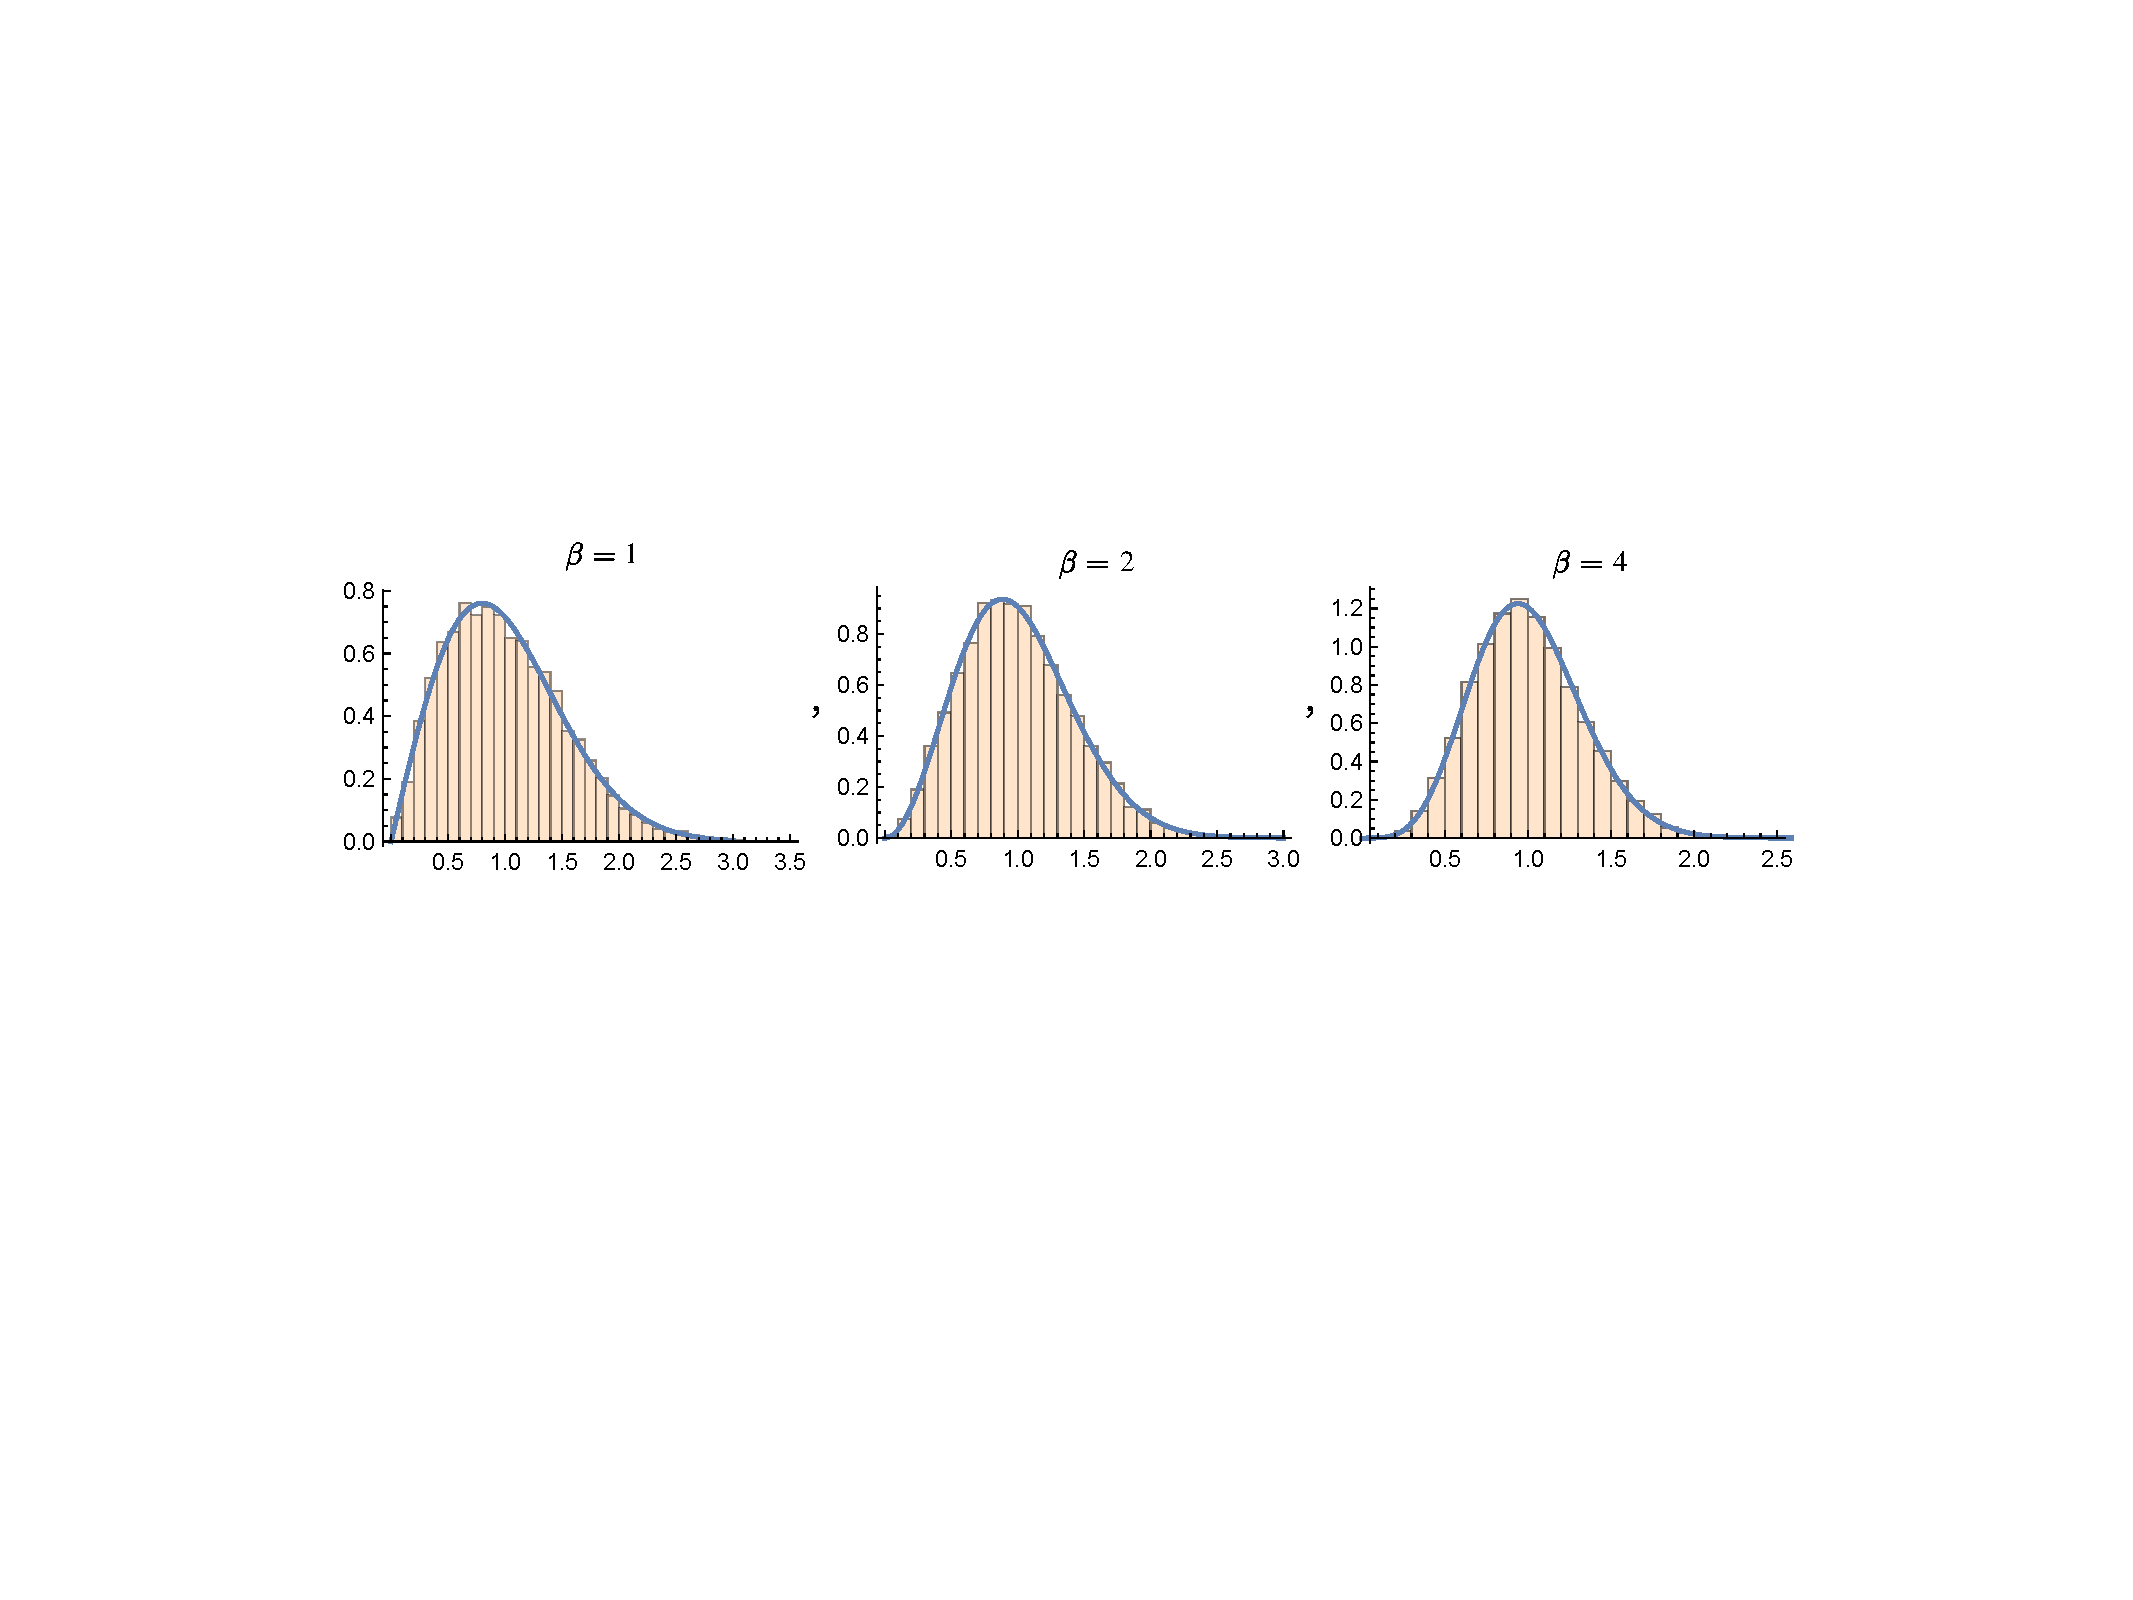
\includegraphics[width=1.05\textwidth]{figs/ensem.pdf}
	\caption{\label{fig:ensem1}The distribution of three ensembles mentioned in the text.}
\end{figure}



\begin{table}[h!]
	\centering
	\begin{tabular}{||c c c||} 
		\hline
		$\beta$ & $c_{\beta}$ & $a_{\beta}$ \\ [0.5ex] 
		\hline\hline
		1 & $\pi s/2$ & $\pi/4$  \\ 
		2 & $32 s^2/\pi^2$ & $4/\pi$  \\
		4 & $2^{18} s^4/3^6 \pi^3$ & $64/9\pi$
		 \\ [1ex] 
		\hline 
	\end{tabular}
\caption{We mention the values for $c_{\beta}$ and $a_{\beta}$ for different ensembles.}
\label{table:c_and_a}
\end{table}


\begin{figure}[htbp] 
	\centering 
	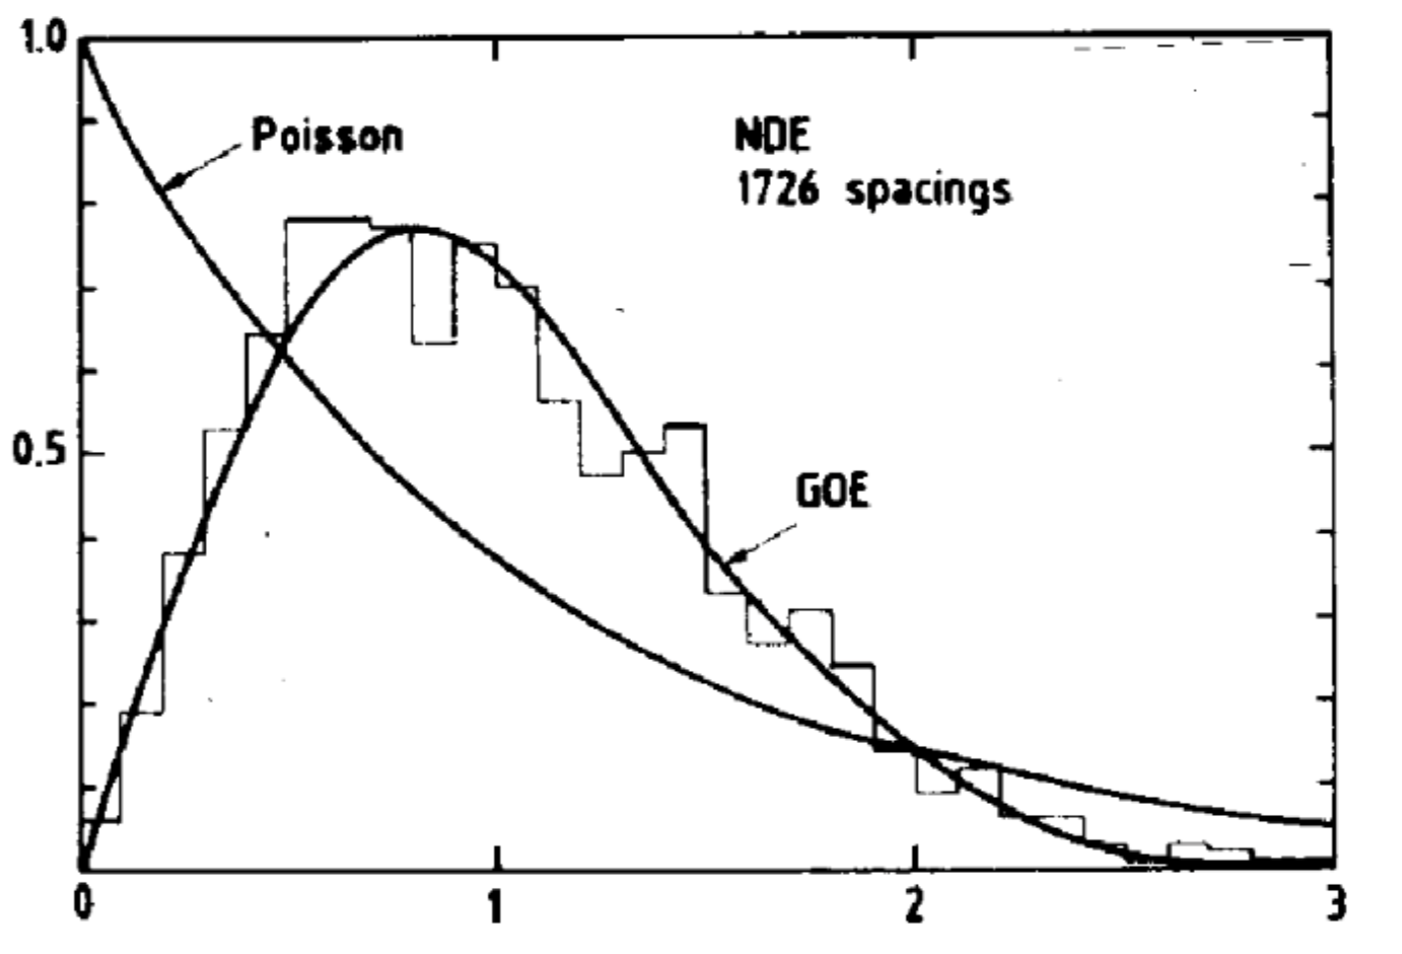
\includegraphics[width=0.55\textwidth]{figs/data_exp.png}
	\caption{\label{fig:data_exp1}The nearest neighbour spacing distribution (i.e., $P(s)$) 
	for nuclear data. The GOE (Gaussian Orthoghonal Ensemble) and Poisson are shown 
	by solid curves. This figure is taken from - ``Fluctuation Properties of Nuclear Energy 
	Levels and Widths : Comparison of Theory with Experiment'' by O. Bohigas, R. U. 
	Haq, and A. Pandey}
\end{figure}

It was later concluded that much to Wigner's own surprise, 
his guess was fairly accurate as shown and improved by Mehta \cite{MEHTA1960395} and 
Gaudin \cite{GAUDIN1961447}. Apart from its extensive use in Physics, the field of random matrix theory is intimately related to areas of Mathematics like number theory 
(especially the pair correlation of the zeros of the Riemann-zeta function) and this was 
observed by Montgomery and Dyson in the 1970s. Some still believe that any future proof of the
Riemann hypothesis lies in the
deepest secrets of random matrix theory. This belief is also the theme of the idea proposed 
independently by  Hilbert and P\'{o}lya who suggested that the zeros of the zeta function 
might be the eigenvalues of some unknown Hermitian `operator'. It is another thing that 
no one yet knows such an operator! We refer the reader to the excellent books 
\cite{Meh2004, Akemann:2011csh} for introductions to the field of random matrix theory. 

The major development in the study of quantum field theories with matrix degrees of freedom satisfyig some well-defined properties started with the work of 't~Hooft in 1974 on the large $N$ limit of gauge theories. By then, it was mostly accepted that the correct theory of 
strong interactions was QCD where we there are matrix degrees of freedom for gauge fields based on $SU(3)$ gauge group. `t Hooft proposed to consider a general $SU(N)$ 
symmetry with large $N$ and he showed that in such a limit only planar diagrams survive and calculations become more tractable and the effects in QCD can be explained as $1/M$ expansion. In fact, this large $N$ limit was later 
understood to be closely related to some description of string theory. This work brought together the idea of random matrix models in the asymptotic limit (large matrices) to mainstream Physics and is extremely fruitful till date. 
This also enabled us to study several interesting features of quantum gravity 
from a field theoretic point of view through the famous AdS/CFT conjecture.
There are some excellent reviews about random matrix theory, matrix integrals/models, large $N$ limit 
and their formal aspects. We refer the reader to two excellent reviews written more than two decades 
apart \cite{DiFrancesco:1993cyw,Eynard:2015aea} for detailed discussions. \\


The goal of this article is to introduce the numerical solutions of matrix models using Monte Carlo (MC) methods and implement them to solve several multi-matrix 
models where no other analytical/numerical treatment is possible in the large $M$ limit. The motivation for this work is partly from the recent progress in the numerical bootstrap program to 
solve matrix models and we hope that these notes with the \PY~ codes will supplement
those explorations and serve as a cross-check of the results. All the codes in these notes can be accessed at:  
\begin{center} \texttt{\href{https://github.com/rgjha/MMMC}{https://github.com/rgjha/MMMC}} \end{center}
The plan of the article is as follows. In Sec.~\ref{sec:MMAres}, we mention saddle-point one-cut solution 
of one matrix Hermitian model and provide a brief explanation about an alternative and equally effective
method of orthogonal polynomials and show how it can be used to 
solve a unitary matrix model. We provide some additional details about Ising model on random graph 
which was also solved using this method in Appendix~\ref{sec:Ortho_pol1}. 
Then in Sec.~\ref{sec:NSOL}, we start by discussing the recent 
numerical bootstrap results for matrix models and then focus for bulk of the 
remaining section on explaining the basics of MC method and use it to solve different models. 
We hope on how the close association between MC 
and bootstrap can serve as a useful guide to solve matrix models. 


\section{\label{sec:MMAres}Matrix models - Analytical results} 
Matrix models (or matrix integrals) are the simplest of models in Physics 
defined with integration over matrices in zero dimensions. 
In these cases, one evaluates integrals of the form:
\begin{equation}
Z = \int dM_{i} \cdots dM_{j} \exp\Bigg[-N \mathrm{Tr} \sum V(M_{i})\Bigg] 
\end{equation}
where $M_{i}$ are $N \times N$ complex matrices which can either be hermitian or unitary.  
In the study of zero-dimensional gauge theories, we encounter these types of matrix models 
where the integral is over the Haar measure. These models often have interesting features in the 
large $N$ limit. In following subsections, we discuss two matrix models and mention two different methods in which they both can be respectively solved.

\subsection{One-matrix model with cubic and quartic potentials - Saddle point analysis}
Before we delve into the details of how to solve the one matrix model using the 
saddle point (or `stationary phase') method, we discuss the basics of this in a simple setting where we deal with integrals over a large number $N$ of variables. Suppose we want to evaluate the integral given by:

\begin{equation}
\label{eq:SP1} 
I(\alpha) = \lim_{\alpha \to 0} \int_{-\infty}^{\infty} e^{-\frac{1}{\alpha}f(x)} ~dx, 
\end{equation}
where $\alpha$ is a positive integer but we would like to eventually consider the interesting limit 
of $\alpha \to 0$ and $f(x)$ is a real valued function. In the limit where $\alpha$ becomes small, 
the exponential causes the integrand to peak sharply at the function's minima. There might be several extrema,
But the integral will be dominated by one which minimizes $f(x)$ as $\alpha \to 0$ (let it be $x_{0}$), 
we use the Taylor expansion about the saddle point $x_{0}$ and throw away higher-order terms to get:
\begin{equation}
	\label{eq:sad_sol2}
	f(x) = f(x_{0}) + f^{\prime\prime}(x_{0}) (x-x_0)^{2} + \cdots 
\end{equation}
Using (\ref{eq:sad_sol2}) in (\ref{eq:sad_sol1}) along with the famous Gaussian integral result i.e.,  $\int_{-\infty}^{\infty} e^{-\alpha x^2} dx = \sqrt{\frac{\pi}{\alpha}}$ we get the desired result:

\begin{equation}
	\label{eq:sad_sol1} 
	I(\alpha) =  \sqrt{\frac{2\pi \alpha}{f^{\prime\prime}(x_{0})}} e^{-f(x_{0})/\alpha}. 
\end{equation}



\begin{mdframed}[backgroundcolor=blue!3] 
	\textsc{} 
	$\bullet$ Exercise 1: Find the terms which are of $\mathcal{O}(\alpha)$ in (\ref{eq:SP1}) by doing little more work and show that:
	\begin{equation*}
	I(\alpha) = \int_{-\infty}^{\infty} e^{-\frac{1}{\alpha}f(x)} ~dx = \sqrt{\frac{2\pi \alpha}{f^{\prime\prime}(x_{0})}} e^{-f(x_{0})/\alpha} \Bigg[1 + 
	\Big[ \frac{5}{24} \frac{(f^{\prime\prime\prime})^2}{(f^{\prime\prime})^3} - \frac{3}{24} \frac{f^{\prime\prime\prime\prime}}{(f^{\prime\prime})^2}\Big] \alpha + \mathcal{O}(\alpha^{2})\Bigg]. 
	\end{equation*}	
\end{mdframed} 

The one matrix hermitian model using the saddle point method was famously solved by Brezin-Itzykson-Parisi-Zuber (BIPZ) \cite{Brezin:1977sv}. This solution is standard and can be found in any standard review or textbooks 
\cite{DiFrancesco:1993cyw, Marino:2004eq}. 
This model is solved using the method of resolvent
and we will briefly sketch the solution described below:
\begin{align}
	Z &= \int dM \exp\Big[-N~\mbox{Tr} V(M)\Big] \\
	& = \int \prod d\lambda_{i} \Delta^2(\lambda)  e^{-N \sum V(\lambda_i)} 
\end{align}
where $\Delta(\lambda) = \prod_{i > j} (\lambda_i - \lambda_j) = \exp\Big[\sum_{i>j} \log |\lambda_{i} - \lambda_{j}|\Big]$ is the Vandermonde 
determinant. If we vary one of the eigenvalues, it gives the saddle point equation:
\begin{equation}
	\label{eq:v_saddle}
	\frac{2}{N} \sum_{j \neq i} \frac{1}{\lambda_i - \lambda_j} = V^{\prime}(\lambda_i).
\end{equation}
It is useful to introduce the density of eigenvalues,
\begin{equation}
	\rho(\lambda) = \frac{1}{N} \sum_{i=1}^{N} \delta(\lambda - \lambda_i). 
\end{equation}
In the limit of large $N$, we can write (\ref{eq:v_saddle})
as:
\begin{equation}
	\label{eq:vprime}
	V^{\prime}(\lambda) = 2 \fint d\mu \frac{\rho(\mu)}{\lambda - \mu} 
\end{equation}
where by $\fint$ we meant the Cauchy principal value of the integral. For often deal with symmetric single-cut such that $b=-a$. We can write resolvent by noting that it is the Stieljes transform of the eigenvalue density as: 

\begin{equation}
	G(z) = \fint d\mu \frac{\rho(\mu)}{\mu - z}
\end{equation}
which we can then write using Sokhotski-Plemelj theorem,
%\footnote{This theorem is $\lim_{\epsilon \rightarrow0} 
%\int_a^b\frac{f(x)}{x+i\epsilon}dx=-i\pi f(0)+ \text{PV}\int_a^b\frac{f(x)}{x}dx$, where PV is the principal value}):
\begin{equation}
	G(z \pm i \epsilon) = \fint d\mu \frac{\rho(\mu)}{\mu - z} \mp i\pi \rho(z),  
\end{equation}
and is equivalent using (\ref{eq:vprime}) to: 
\begin{equation}
	G(z \pm i \epsilon) = -\frac{1}{2} V^{\prime}(z) \mp i\pi \rho(z).  
\end{equation}
Once we find the resolvent, we can solve the model and find the moments through the eigenvalue density. 
It is useful to mention here that we can use the useful closed expression for 
resolvent in terms of a contour integral (see for example (A.24) of \cite{Migdal:1983qrz})
as given by:
\begin{equation}
	G(x) = \int_{-a}^{a} \frac{-1}{2\pi i} \frac{\sqrt{x^2-a^2}}{\sqrt{y^2-a^2}} N V^{\prime}(y) \frac{1}{x-y}, 
\end{equation}
for symmetric `one-cut' solutions and by,
\begin{equation}
	G(x) = \int_{b}^{a} \frac{-1}{2\pi i} \sqrt{\frac{(x-a) (x-b)}{(y-a)(y-b)}}  N V^{\prime}(y) \frac{1}{x-y} dy, 
\end{equation}
if the cut was instead $[b,a]$. For the case of 1MM with quartic potential i.e., 
$V(M) = M^2/2 + gM^4/4$, one obtains the exact result (for $g \ge -1/12$):
\begin{equation}
\label{eq:exact1MM} 
t_{2} = \frac{(12 g+1)^{3/2}-18 g-1}{54 g^2}. 
\end{equation}
The \MA~code to solve this model is given in Appendix~\ref{sec:math_code} for the convenience of the reader. 


\begin{mdframed}[backgroundcolor=blue!3] 
	\textsc{} 
	$\bullet$ Exercise 2: Show that $\det(V) = \prod_{i<j} (\lambda_i - \lambda_j)$ where $V$ is given by: 
	\begin{equation*}
		V = 
		\begin{pmatrix}
			1 & \lambda_1 & \lambda_{1}^{2} & \cdots & \lambda_{1}^{N-1} \\
			1 & \lambda_2 & \lambda_{2}^{2} & \cdots & \lambda_{2}^{N-1} \\ 
			\vdots  & \vdots  & \ddots & \vdots  \\
			1 & \lambda_N & \lambda_{N}^{2} & \cdots & \lambda_{N}^{N-1} 
		\end{pmatrix} = \lambda_{i}^{j-1} 
	\end{equation*}
	
\end{mdframed} 

\begin{mdframed}[backgroundcolor=blue!3] 
	\textsc{} 
	$\bullet$ Exercise 3: Derive the loop equations (aka Schwinger-Dyson equations) given below: \\ 
	\begin{equation}
		\label{eq:LE1} 
		\Big< \mbox{Tr} M^{k} V^{\prime}(M) \Big> = \sum_{l=0}^{k-1} \langle \mbox{Tr} M^{l} \rangle  \langle \mbox{Tr} M^{k-l-1} \rangle
	\end{equation} 
\end{mdframed}

\subsection{One-plaquette unitary model - Orthogonal polynomials} 

The origin of large $N$ limit of gauge theories was motivated by the hope of understanding 
the accepted theory of strong interactions (QCD). 
In the subsequent years, ~t~Hooft solved two-dimensional model of mesons in large $N$ 
limit. One of the first known examples of a unitary matrix model which was relevant to lattice gauge theory (and to QCD) was considered by Gross, Witten, and Wadia (GWW) \cite{Gross:1980he, Wadia:2012fr}.
This is often known as one-plaquette matrix model and describes the gauge part of large $N$ of the two-dimensional Yang-Mills theory (also sometimes called $\rm{QCD}_{2}$).
This model also has deep connections to string theory in the so called `double-scaling limit' (DSL) where $N \to \infty$ and $\lambda \to \lambda_{c}$ simultaneously. 
The requirement of this double scaling can be understood as follows: 
If we merely take $N \to \infty$ then we get genus zero surfaces in the 
expansion of the free energy. However, this would prohibit string interaction 
since they would imply a change of genus which is not possible in that limit. 
In taking DSL, this problem is resolved and topological information is maintained. 
It is given by the partition function: 
\begin{equation}
	Z = \int \exp \Big[- \mbox{Tr} (U + U^{\dagger})   \Big] dU. 
\end{equation}
This model admits exact solution for all $N$ and $\lambda$ in terms of determinant of a 
Toeplitz matrix. However, it is not very useful and hence this model has been studied by 
saddle-point methods and orthogonal polynomials (OP). We will sketch the solution using OP 
closely following \cite{Goldschmidt:1979hq}. 
Following the discussion in the Appendix~\ref{sec:Ortho_pol1}, we define the polynomial:
\begin{equation}
	P_{j}(x) = \sum_{k=0}^{j-1} b_{k} x^{k} + x^{j}. 
\end{equation} 
We have to choose polynomials that are orthonormal with respect to the measure which in this case is:
\begin{equation}
	\rho(\theta) = \exp\Big[\frac{2N}{\lambda} \cos \theta \Big],
\end{equation}
and this results in:
\begin{equation}
	\int_{-\pi}^{\pi} \rho(\theta) P_{m}(e^{i\theta}) P_{n}^{*}(e^{i\theta}) = a_{m} \delta_{mn}
\end{equation}
If we define $\kappa = 2N/\lambda$, then we have for the representation in terms of 
Bessel functions as, 

\begin{equation}
	I_{n}(\kappa) = I_{-n}(\kappa) = \int_{-\pi}^{\pi} \rho(\theta) e^{i n \theta}, 
\end{equation}
and the polynomials defined above becomes:
\begin{equation}
	P_{n}(z) = \det
	\begin{pmatrix}
		I_0 & I_1 & \cdots & I_n \\
		I_1 & I_0 & \cdots & I_{n-1} \\
		\vdots  & \vdots  & \ddots & \vdots  \\
		1 & z & \cdots & z^n 
			\end{pmatrix}
		 \frac{1}{\det [I_{i-j} (\kappa)]_{i,j = 1 \cdots N}}
\end{equation}.
We note that the coefficients of $P_{n}(z)$ are real and hence $P_{n}^{*}(e^{i\theta}) = P_{n}(e^{-i\theta})$. It is also starightforward by expanding the determinant to see that: $a_{n} = c_{n+1}/c_{n}$ where $c_{n} = \det [I_{i-j}(\kappa)]_{i,j = 1 \cdots n}$ is the Toeplitz determinant. 
In fact, it is easy to show that for this U($N$) model, $Z$ is just $c_{n}$ (i.e., only single coefficient remains in (\ref{eq:ZOP})) and we get, 
\begin{equation}
\label{eq:GWW_ex} 
Z = \det \Big[I_{i-j}(\kappa) \Big].
\end{equation}
The result is true for all $\lambda$ and $N$. If we impose additional constraint of 
$U$ belonging to the $SU(N)$ rather than $U(N)$ group, it is easy to show that
it becomes:
\begin{equation}
\label{eq:GWW_ex} 
Z = \sum_{k=-\infty}^{\infty} \det \Big[I_{i-j+k}(\kappa) \Big].
\end{equation}
%\subsection{Open and closed $p$-matrix chain model}
In addition to this model, there are many other interesting matrix models which can be solved analytically
and are physically relevant which we will not discuss here. 
One such model is the external field problem which was considered in \cite{Brezin:1980rk}. In this paper, a matrix 
model of unitary links was solved with an external field in the large $N$ limit and found to have a third-order phase transition. These models are relevant for several problems in lattice gauge theory. This model reduces to the GWW model when the external source is set to unit matrix. These developments in large $N$ $\rm{QCD}_{2}$ models also lead after few years to the idea of volume reduction in large $M$ limit known as Eguchi-Kawai volume reduction \cite{Eguchi:1982nm}. They showed that in planar limit, the lattice gauge theory for an infinite lattice and unit cube are identical. The space-time seems incorporated in the large $N$ limit as an internal degree of freedom. There are some subtlety involved but this has lead to interesting work, see Ref.~\cite{Kovtun:2007py} for instance. 

%\vspace{20mm}  
\section{\label{sec:NSOL}Numerical solutions} 
There is only a selected list of analytically solvable matrix models in the planar limit. This inevitably brings 
the thought of attempting numerical solutions. Unfortunately, even here, there are not many methods 
which one can use. In fact, there are only two methods with the second method barely few years old! 
This clearly signals the fact that there still remains a lot of work to be done in devising new numerical 
methods to solve matrix models. The most frequently used method is Monte Carlo (MC)\footnote{
It is not widely known that Monte Carlo methods were central to the work required for the Manhattan Project
and first introduced in the 1940s by Stanislaw Ulam and recognized first by Von Neumann. 
He is often credited as the inventor of the modern version of the Markov Chain Monte Carlo 
method. In fact, the earliest use of MC goes back to the solution of the Buffon needle problem when Fermi used it in the 
1930s but never published it. 
Since this work was part of the classified information, the work of von Neumann and Ulam required a code name. It was Metropolis who 
suggested using the name Monte Carlo based on the casino in 
Monaco where Ulam's uncle would borrow money from relatives to gamble. Ulam and Metropolis
published the first paper on MC in 1949 titled `The Monte Carlo Method'.} 
is quite effective but is not a panacea. 
The newly introduced numerical bootstrap method has already been used to solve several matrix models \cite{Anderson:2016rcw,Lin:2020mme,Han:2020bkb,Kazakov:2021lel} but the extension to matrix models with more than two matrices i.e., 3-matrix commutator type models or IKKT models seems highly non-trivial at the moment. 
This is related to the fact that with more matrices, the loop equations which become highly non-linear are difficult to handle.
In these notes, we will mostly focus on MC methods since as of this writing bootstrap methods have not been able to access or constrain matrix models with more than two matrices. However, we want to explain the bootstrap solution for the case of one matrix model as first shown by \cite{Lin:2020mme} for the interested reader. For a detailed exposition, we refer the reader to the references above. 
We hope that this yet small section on bootstrap methods would be extended in later versions 
of these notes as more results accumulate in coming years. 

\subsection{Matrix bootstrap method}
The basic idea of bootstrapping matrix models depends on the 
positivity (positive-definiteness) of the bootstrap matrix which we refer in what follows 
by $\mathcal{M}$. For the case of one matrix model (1MM) with a potential $V(X)$ given by: 
\begin{equation}
    V(X) = \frac12 X^2 + \frac{g}{4} X^4, 
\end{equation}
the odd moments of X vanishes i.e., $ t_{n} = (1/N)\mbox{Tr} X^n = 0$ for odd $n$
while the even moments (of order greater than two) are all related to $t_{2}$. This renders the 
model simple to bootstrap since there is no growth of words (combination of matrix or matrices!)
since all non-zero $t_{n}$ can be related to $t_{2}$. 
\begin{mdframed}[backgroundcolor=blue!3] 
	\textsc{} 
	$\bullet$ Exercise 4: Use loop equations and show that for the 1MM with quartic potential, it is possible to write $t_{4}, t_{6}, t_{8}$ in terms of $t_{2}$. Also, check this either using \MA~ or \PY~ [see Appendix for details]. 
Repeat this exercise for cubic potential where higher moments can be written in terms of $t_1$.  
\end{mdframed} 
If we consider positive constraints that can be derived from $\langle \mbox{Tr}(\Phi^{\dagger}\Phi) \rangle \ge 0 $
where $\Phi$ is a superposition of matrices which for one matrix model is 
$ \Phi = \sum_{k} \alpha_{k} M^{k}$. This condition is equivalent to the positive definite nature of
$\mathcal{M} \succeq 0 $ where $ \mathcal{M}_{ij} = \langle \mbox{Tr} M^{i+j} \rangle$. 
We can only enforce a subset of these constraints. For example, it was sufficient to 
access the positive definite nature of $\mathcal{M}_{6 \times 6} \succeq 0 $ 
and sub-matrices to get to the exact solution in Ref.~\cite{Lin:2020mme}. 
For example, $\mathcal{M}_{2 \times 2}$ is given by:
\begin{equation}
	\mathcal{M}_{jk} = 
	\begin{pmatrix}
		t_{2j} & t_{j+k}  \\
		t_{j+k} & t_{2k}  
	\end{pmatrix}  \succeq 0
\end{equation}
In this case, solving the model just means finding the bounds on $t_{2}$ 
since all others can then be calculated (see the exercise above). 
Following this work, a quantum mechanics 
model (in 0+1-dimensions) with two matrices was solved using similar techniques. 
The results obtained were shown to be consistent with MC results. 
In this work, the Hamiltonian considered was given by:
\begin{equation}
H = \mbox{Tr} \Big( P^2 + X^2 + \frac{g}{N} X^4 \Big)
\end{equation}
and corresponding to the trial operators up to length (L) = 2, 
they considered $ \mathbb{I}, X, X^{2}$ and $P$. The bootstrap matrix
of size $2^L \times 2^L$ which should be positive definite is constructed as:

\begin{equation}
	\mathcal{M} = 
	\begin{pmatrix}
		\langle \mbox{Tr}\mathbb{I} \rangle & \langle \mbox{Tr} X^2 \rangle & 0 & 0 \\
		\langle \mbox{Tr} X^2 \rangle & \langle \mbox{Tr} X^4 \rangle  & 0 & 0 \\ 
		0 & 0 & \langle \mbox{Tr} X^2 \rangle & \langle \mbox{Tr} XP \rangle \\
		0 & 0  & \langle \mbox{Tr} PX \rangle & \langle \mbox{Tr} P^2 \rangle
	\end{pmatrix}  \succeq 0
\end{equation}
They considered bootstrap matrices up to $L=4$ and observed
convergence to the expected result. 
For the case of two-matrix quantum mechanics, the convergence
was found to be slow but consistent with results expected using Monte Carlo results and bounds from Born-Oppenheimer wavefunction. Another two-matrix integral model given by the action (\ref{eq:GHM1}) was recently solved \cite{Kazakov:2021lel}. 
In this work, authors used relaxation bootstrap methods (which takes us 
from non-linear semi-definite programming (SDP) problem to linear) with
$\Lambda=11$ (which determines the size of the minor of the full bootstrap matrix) 
to constrain the moments of matrices such as $\mathrm{Tr}X^2/N = t_{2}$ and $t_{4}$ 
to five decimal places for the symmetric case. We will come back to 
discuss this model for both symmetric and symmetry broken cases 
and its corresponding solution using MC methods in Sec.~\ref{subsec:Hoppe}. 
and show that they are in perfect agreement.  

\subsection{Monte Carlo method}
The numerical method which is state-of-the-art in classical computations 
of matrix models and quantum field theories in general is the Monte Carlo approach.
For higher-dimensional models, one starts with the lattice formulation which reduces the 
path-integral introduced by Feynman into many ordinary integrals. But even for a simple
gauge theory like $\mathbb{Z}_{2}$ in four dimensions, this is not practical to evaluate. 
The fact that we need to do so many integrals suggests that may be some statistical 
interpretation and this is where the basic idea of Monte Carlo comes in. It selects the 
configuration which dominates the path integral and then ignores the rest of the available
phase space and only focuses on this important sampling. In this way, one constructs a chain of configurations 
that approximately leads to the required distribution. 
Metropolis-Hastings algorithm and Hamiltonian/Hybrid Monte Carlo (HMC) 
are two frequently used methods that
can generate a Markov chain and lead to unique stationary distribution. 
We will here focus on the latter since that has now become the state-of-the-art in 
various numerical computations. This method was introduced in 
1987 by Duane, Kennedy, Pendleton, and Roweth \cite{Duane:1987de} who put together the ideas from
Markov chain Monte Carlo (MCMC)\footnote{MCMC originated in the seminal paper of 
Metropolis et al.~\cite{Metropolis:1953am}, where it was used to simulate the state distribution for a system of ideal molecules.} 
and molecular dynamics (MD) methods. 
For a detailed review about HMC and its extension to rational 
HMC which is required for fermions, the interested readers 
can consult the Refs. \cite{Hanada:2018fnp,Joseph:2019zer}. 
The two basic parts of HMC are, a) Use of integrator to evolve and propose a new configuration, b) accept or reject
the proposed configuration. But before we discuss HMC, 
it is important to see how we generate random momentum 
matrices for the leapfrog algorithm 
at the start of each trajectory (time unit) since 
this is necessary to ensure that we converge to the 
correct answer using Monte Carlo methods. 


\subsubsection{Random number generator}  
%%%%%%%%%%%%%%%%%%%%%%%%%%%%%%%%%

It is essential during a Monte Carlo process that we correctly generate momentum matrices at the start of the leapfrog method taken from a Gaussian distribution. In this part, we will sketch this process and provide the accompanying code. 
Suppose we have two numbers $U$ and $V$ taken from uniform distribution i.e., (0,1) 
and we want two random numbers with probability density function $p(X)$ and $p(Y)$ given by:
\begin{equation}
	p(X) = \frac{1}{\sqrt{2\pi}} e^{-X^2/2} 
\end{equation}
and, 
\begin{equation}
	p(Y) = \frac{1}{\sqrt{2\pi}} e^{-Y^2/2} 
\end{equation}
Since $X$ and $Y$ are independent, we can write:
\begin{equation}
	p(X,Y) = p(X) p(Y) = \frac{1}{2\pi} e^{-R^2/2} = p(R, \Theta) 
\end{equation}
where $R = X^2 + Y^2$. This allows us to make the following identification:
\begin{equation}
	U = \frac{\Theta}{2\pi}, 
\end{equation}
and, 

\begin{figure}[htbp] 
	\centering 
	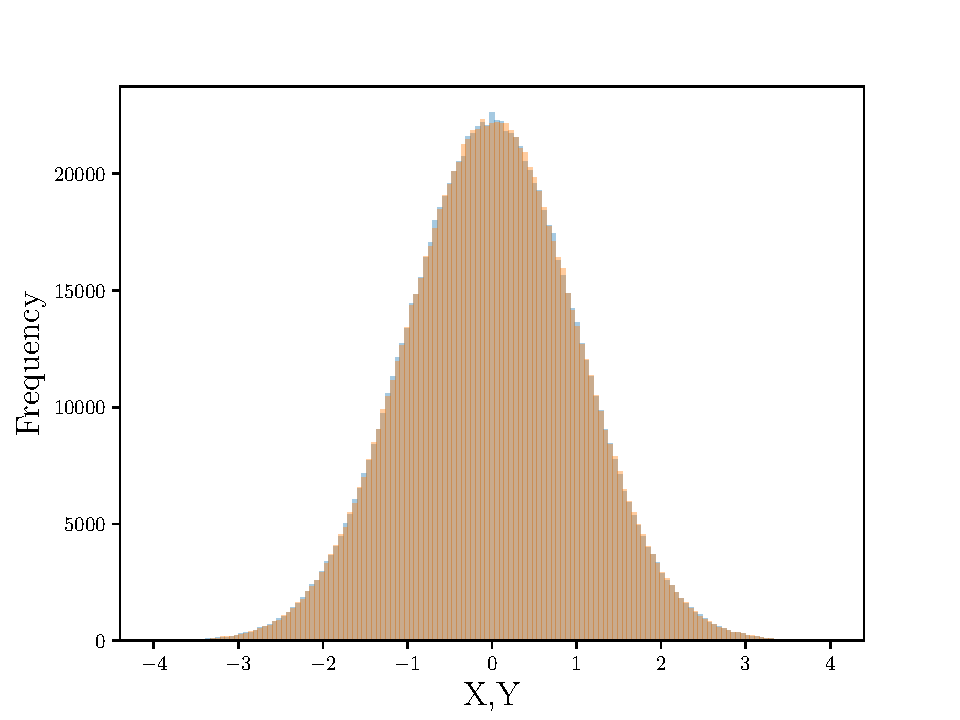
\includegraphics[width=0.75\textwidth]{figs/testRN.pdf}
	\caption{\label{fig:RN}In the limit of large sample size (here 1 million), 
	it tends to Gaussian with mean zero and $\sigma=1$. For example, if 
	this was not true then the MC results would converge to an incorrect answer.}
\end{figure}
\begin{equation}
	V = e^{-R^2/2} \implies R = \sqrt{-2 \log(V)}. 
\end{equation}
This implies, 
\begin{align}
	X &= R \cos \Theta = \sqrt{-2 \log(V)} \cos(2 \pi U), \\
	Y &= R \sin \Theta = \sqrt{-2 \log(V)} \sin(2 \pi U).
\end{align}
The code to implement this in \PY~ is given below: 
\begin{mdframed}[backgroundcolor=mauve!3] 
\begin{lstlisting}[language=Python]
def box_muller():  
# Basic form (alt: polar form) of Box-Muller random number generator for pairs of 
# independent, standard, normally distributed (mean=0, sigma=1) 
# given a source of uniformly distributed random numbers in (0,1)
# p, q have weights exp(-p^2/2)/sqrt(2pi) and exp(-q^2/2)/sqrt(2pi) respectively. 

    PI = 2.0*math.asin(1.0);    
    r = random.uniform(0,1)
    s = random.uniform(0,1)
    x = np.sqrt(-2.0*np.log(r)) * math.sin(2.0*PI*s)
    y = np.sqrt(-2.0*np.log(r)) * math.cos(2.0*PI*s)
    return x,y
\end{lstlisting}
\end{mdframed} 
It is easy to check that it indeed generates a 
Gaussian distribution with desired properties as shown in Fig.~\ref{fig:RN}. 

\subsubsection{Leapfrog integrator and Metropolis step}
The leapfrog method (also sometimes known as `hopscotch' method) 
is used to numerically integrate differential equations. This is a second-order 
method and the energy non-conservation depends on the square of step-size used. This integrator is `symplectic', i.e., it preserves the 
area of the phase space. We can understand this as follows: 
Consider a rectangular region of area $dA$ as shown below in Fig.~\ref{fig:PSP1}. The four corners at time $t$ are denoted by $(x, p), (x+dx, p), (x+dx, p+dp),(x, p+dp)$. At some later time $t^{\prime}$, this will change to form corners of some quadrilateral as shown with area $dA^{\prime}$. It is then the statement of Liouville's theorem\footnote{Note that Liouville theorem is closely related to detailed balance condition which says that in equilibrium there is balance between any two pairs of states i.e., equal probability.} that the areas are equal, i.e., $dA = dA^{\prime}$. 
\begin{figure}[htbp] 
	\centering 
	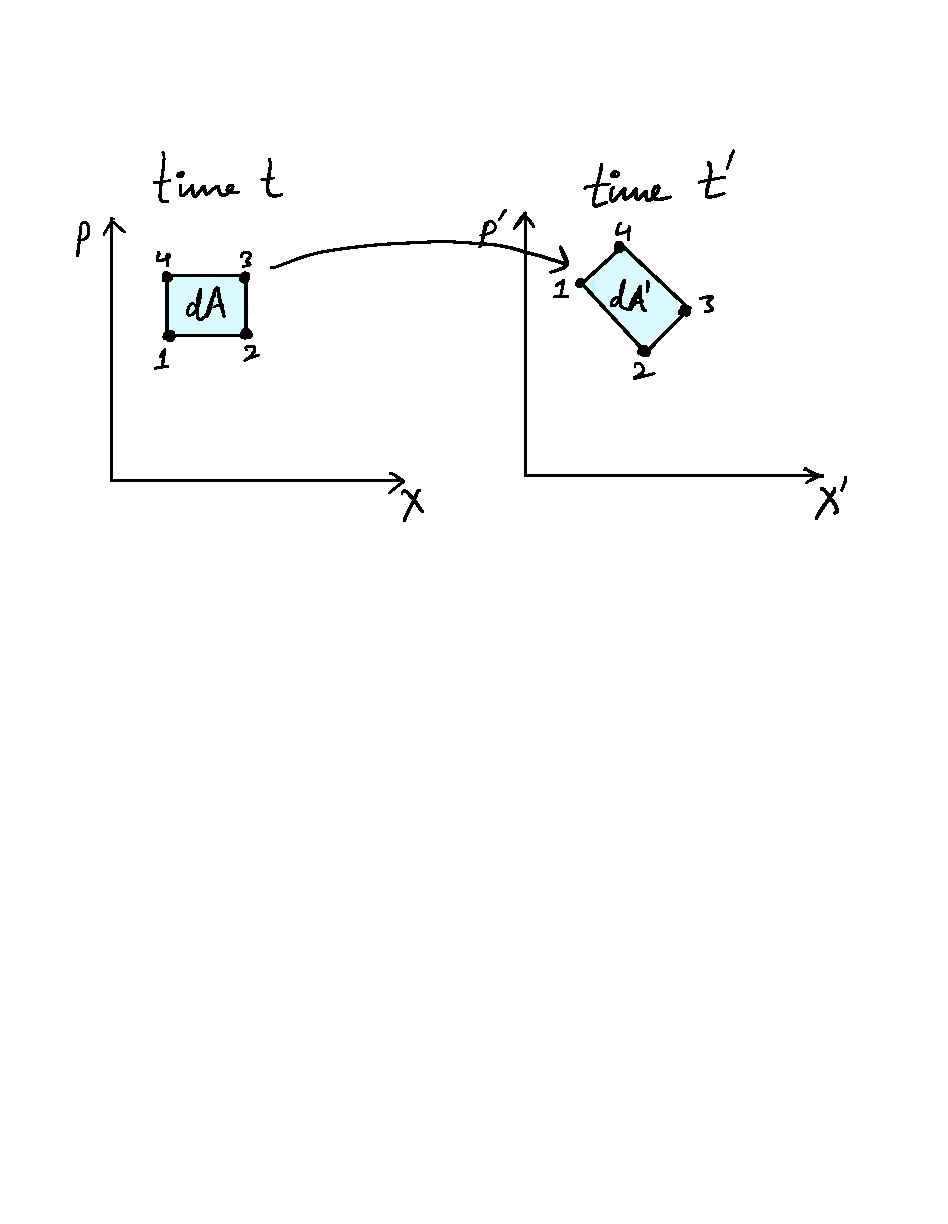
\includegraphics[width=0.75\textwidth]{figs/PSP.pdf}
	\caption{\label{fig:PSP1}A representation of conservation of phase space area. It asserts that under the evolution of the system, it may change the shape of the shaded region but not the volume since probability must be conserved.}
\end{figure}
Using this idea we can easily prove important equality used to check various lattice computations employing symplectic integrators left as an exercise for the reader. The basic steps of the leapfrog algorithm are as follows:
\begin{itemize}
	\item $X_{i}\big(\frac{\Delta \tau}{2}\big) = X_{i}(0) + P_{i}(0)\frac{\Delta \tau}{2}$
	\item Now several inner steps where $n =  1 \cdots (N-1)$
	\subitem $P_{i}(n \Delta \tau) = P((n-1) \Delta \tau) - f_{i}((n-\frac{1}{2}) \Delta \tau) \Delta \tau$ 
	\subitem $X_{i}((n + 1/2) \Delta \tau) = X_{i}\Big(\Big(N - \frac{1}{2}\Big) \Delta \tau\Big)  + P_{i}(n \Delta \tau) \Delta \tau$
	\item $P_{i}(N \Delta \tau) = P_{i}((N-1) \Delta \tau) - f_{i}((N-\frac{1}{2}) \Delta \tau) \Delta \tau$ 
	\item $X_{i}(N \Delta \tau) = X_{i}\Big(\Big(N - \frac{1}{2}\Big) \Delta \tau\Big) + P_{i}(N \Delta \tau) \frac{\Delta \tau}{2}$ 
\end{itemize} 
    \begin{mdframed}[backgroundcolor=blue!3] 
    \textsc{} 
    $\bullet$ Exercise 5: Show that a consequence of Liouville theorem is that $ \langle e^{-\Delta H(\boldsymbol{\cdot})} \rangle = 1$, where $\boldsymbol{\cdot}$ denote fields. Check this also holds in any given HMC simulation within errors if a symplectic integrator is used and we ignore proper data for thermalization cut.
    \end{mdframed} 
In the last step of HMC, a Metropolis test is carried out to accept or reject the proposed
configuration. Suppose we start from the configuration $X$ of a one matrix model 
which is a $N \times N$ matrix and carry out the leapfrog part with some parameters and obtain a new configuration 
$X^{\prime}$. The test then computes \texttt{$\text{min.}(1, e^{-\Delta H})$} and generates 
a uniform random number between $r \in [0,1]$. The new configuration is 
rejected if \texttt{$\text{min.}(1, e^{-\Delta H}) < r$} otherwise accepted. 


%%%%%%%%%%%%%%%%%%%%%%%%%%%%%%%%%
\subsubsection{Autocorrelation and jackknife errors} 

It must be kept in mind that given a Markov chain, the new states 
(i.e., configurations) can be highly correlated to previous ones. 
In order to ascertain that the measurement of an observable $\langle \mathcal{O} \rangle$ is not affected by correlated configurations, it is essential for proper statistical analysis to know the extent to which they are correlated. In this regard, it is important to measure
the autocorrelation time $ \tau_{\rm{auto}}$ which measures the time it takes for two measurements to be considered independent of each other. So, if we generate $L$ configurations, then actually only $L/\tau_{\rm{auto}}$ are useful for computing averages.
We define the autocorrelation function of observable $\mathcal{O}$ as:
 
 \begin{equation}
 	C(t) = \frac{\langle \mathcal{O}(t_0) \mathcal{O}(t_0 + t) \rangle - \langle \mathcal{O}(t_0)\rangle \langle \mathcal{O}(t_0 + t) \rangle}{\langle \mathcal{O}^2(t_0)\rangle - \langle \mathcal{O}(t_0)\rangle^{2}}
 \end{equation}.
The behaviour of $C(t)$ is $\sim \exp(-t/\tau_{\rm{auto}})$ as $ t \to \infty$. This is called exponential autocorrelation time. We can also compute something which is called `integrated autocorrelation time' defined as:
\begin{equation}
	\tau_{\rm{auto}}^{\rm{int.}} = \frac{\sum_{t=1}^{\infty} \langle \mathcal{O}(t_0) \mathcal{O}(t_0 + t) \rangle - \langle \mathcal{O} \rangle^2 }{\langle \mathcal{O}^2\rangle - \langle \mathcal{O}\rangle^{2}}
\end{equation}.
We can write this in terms of a sum over autocorrelation function as: $\tau_{\rm{auto}}^{\rm{int.}} = 1 + \sum_{t=1}^{N} C(t)$. In general, $ \tau_{\rm{auto}}$ increases with system size, close to the critical point. One 
can express the statistical error in the average of $\mathcal{O}$ denoted 
by $\delta \mathcal{O}$ is given in terms of variance and integrated autocorrelation time as:

\begin{equation}
	\delta \mathcal{O} = \sigma \sqrt{\frac{2 \tau_{\rm{auto}}^{\rm{int.}}}{N}}  %^{\rm{int.}}}{}
\end{equation}
where we have usual definitions i.e., 
$\sigma = \sqrt{\langle \mathcal{O}^2\rangle - \langle \mathcal{O}\rangle^{2}}$ and $N$ is the number of measurements. 

\subsection{One-matrix model with quartic \& cubic potentials: Confirming exact results} 
With a quick introduction of the basic elements of the MC method, we want to use it to study matrix models. For this purpose, 
the exact solution for one matrix model is a good testbed to check numerical results and compare to other different approaches. 
We start off with the quartic potential given by:
\begin{equation}
	V(M) = \frac{M^2}{2} + \frac{gM^4}{4}.  
\end{equation}
As we already mentioned in the section before, this has an exact solution and moments, $t_{n}$ 
can be obtained using the \MA~ code given in the appendix. We show that the exact result and the 
Monte Carlo results agree for $g=1$ in Fig. \ref{fig:1MM_res}. The \PY~ code which was used for this 
can be found in the Appendix~\ref{sec:1MMPYC}. In the appendix, we also 
discuss how to run the code on your laptop and the estimated time to completion. The most recent version of this 
code\footnote{Please email the author for any bug report or additional requests} is available at:
\begin{center} \texttt{\href{https://github.com/rgjha/MMMC}{https://github.com/rgjha/MMMC}} \end{center}. 
The quartic potential one matrix model has a well-known critical coupling i.e., $ g_{c} = -1/12$. 
We note that MC method is equally effective to detect the critical $g$ for matrix models. 
For example, we obtained correct results for $t_{2}$ as given by \ref{eq:exact1MM} 
until $g_{\rm{min.}} \sim -0.0819$ for $N=300$ but the simulation didn't converge (ran away!) 
for $g = -0.0820$. It took us about 1-2 hours of computer time to 
locate the critical coupling to accuracy of about 
$\sim 0.0014$ (i.e., $g - g_{c} \sim 0.0014$). 
We can always increase $N$ to get a 
more precise result. 
\begin{figure}[htbp] 
	\centering 
	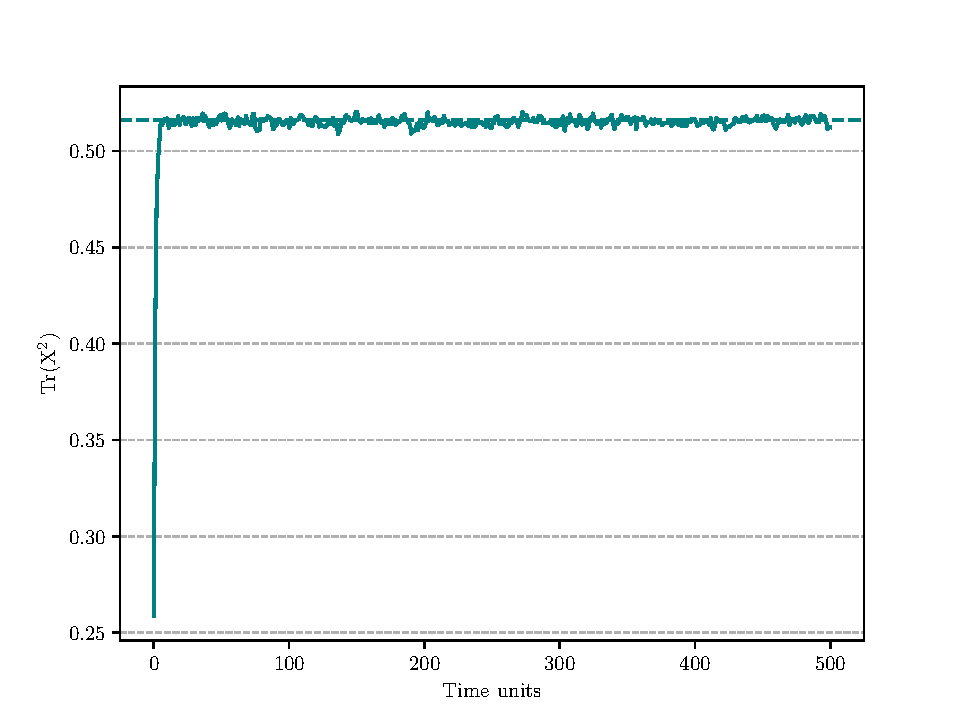
\includegraphics[width=0.75\textwidth]{figs/mm_plot.pdf}
	\caption{\label{fig:1MM_res}The computed value of $\mbox{Tr}(X^2)$ with MC methods for quartic potential
		one matrix model is consistent with that obtained using analytical saddle-point methods (shown by dashed lines). 
		These results are with $N = 300$ and $g = 1$ and took about 40 minutes on a laptop.}
\end{figure}
One can also consider one-matrix model with cubic interaction instead of quartic as above. 
There is well-known instability associated with cubic potential. The potential is given by:
\begin{equation}
	V(M) = \frac{M^2}{2} + \frac{g_{3}M^3}{3}  
\end{equation}
It is only well-defined if $g \le 0.21935$. This is the radius of convergence of the planar perturbation series. 
Though this method can be exactly solved, we encourage the reader to attempt Exercise~6 to numerically solve this using MC. This exercise provides a good practice on how we can modify the potential in the given codes to study another model of interest. 


\begin{mdframed}[backgroundcolor=blue!3] 
	\textsc{} 
	$\bullet$ Exercise 6:  Check that the one matrix model given in the appendix also reproduces the correct result for cubic potential 
	i.e., $V(M) = M^2/2 + g_{3}M^3$.\\  
	\label{ex:6} 
\end{mdframed} 
Another interesting dimer matrix model closely related to the one matrix model was 
studied in the context of understanding the Yang-Lee edge singularity
\cite{Staudacher:1989fy} in Ising model on random graphs. 
It is given by: 
\begin{equation}
	\label{eq:Stau0}
	Z = \int \mathcal{D}X \mathcal{D}M \exp N \mbox{Tr}\Bigg(-\frac{X^2}{2} + \frac{gX^4}{4} - \frac{M^2}{2} + g \sqrt{\zeta} MX^3 \Bigg).
\end{equation}
After integrating out the matrix $M$, we can reduce it to a one matrix model problem, 
\begin{equation}
	\label{eq:Stau1} 
	Z = \int \mathcal{D}X \exp N \mbox{Tr}\Bigg(-\frac{X^2}{2} + \frac{gX^4}{4} + g^2 \zeta  \frac{X^6}{2}   \Bigg)
\end{equation}
Note that if we set $\zeta=0$, this reduces to the 1MM problem but since the sign of 
quadratic term is negative, this is the symmetry broken version of the one matrix model 
discussed above. 
% ax^2 + bx + c -> a(x-h)^2 + k 
% where h = -b/2a and k = c - (b^2/4a)  
\begin{mdframed}[backgroundcolor=blue!3]  
	$\bullet$ Exercise 7: Check that (\ref{eq:Stau1}) follows from (\ref{eq:Stau0}) and modify the potential for the 1MM \PY~code to study this model. 
\end{mdframed} 
% P 706 book
%%%%%%%%%%%%%%%%%%%%%%%%%%%%%%
\subsection{\label{subsec:Hoppe}Hoppe-type matrix models}
% Page 71 of his 1982 thesis. 
We now turn our attention to matrix models with a commutator interaction term. 
To our knowledge, this model 
was first introduced by Hoppe \cite{Hoppe:1982en} and solved later by different methods in 
Refs.~\cite{Kazakov:1998ji,Berenstein:2008eg}.
The partition function is given by:
\begin{equation}
Z = \int \mathcal{D}X \mathcal{D}Y \exp \Big[-N ~ \mbox{Tr} (X^2 + Y^2 - g^2 [X,Y]^2) \Big] 
\end{equation}
At large values of commutator coupling i.e., $ g \to \infty$, this model becomes commuting with 
$ [X,Y] \to 0$. The presence of commutator term in matrix models is common especially in 
models which have a dual gravity interpretation of emergent geometry behaviour. 
The exact result for average action is:
\begin{equation}
	2 \langle S_{c} \rangle + \langle S_{q}  \rangle = N^2 - 1, 
\end{equation}
where $ S_{c} = -Ng^2 \mbox{Tr}[X,Y]^2$  and 
$ S_{q} = N~\mbox{Tr} (X^2 + Y^2) $
This average action serves as a good check of the code. We can alternatively also consider a slightly more 
general two-matrix model which reduces to Hoppe's model mentioned above in a special limit. 
Such a matrix model is generally not solvable. This model was considered in \cite{Kazakov:2021lel} and 
solved using bootstrap methods and is given by:

\begin{equation}
\label{eq:GHM1} 
Z = \int \mathcal{D}X \mathcal{D}Y \exp \Big[-N ~ \mbox{Tr} (X^2 + Y^2 - h^2 [X,Y]^2 + gX^4 + gY^4) \Big].	
\end{equation}

\begin{figure}[htbp] 
	\centering 
	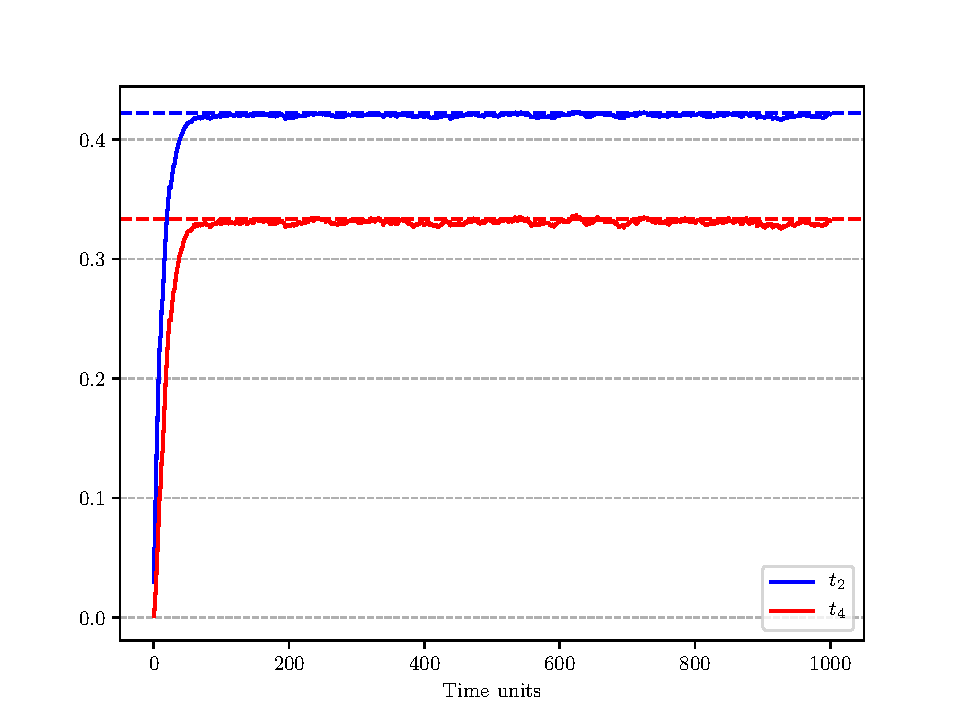
\includegraphics[width=0.75\textwidth]{figs/plot_2MM_sym1.pdf}
	\caption{\label{fig:2MM_match}The matrix model defined by~(\ref{eq:GHM1}) is not solvable and was 
recently studied using bootstrap methods. We show the MC by solid lines and those 
obtained using bootstrap by dashed lines. We get about three digits of accuracy with 1000 time units 
by running for 1.5 hours on the laptop. The results are with $g=h=1$ and $N=300$. For larger $N$ say, $N=800$, 
the same run will take about 16-18 hours.}
\end{figure} 

The action in (\ref{eq:GHM1}) has $\mathbb{Z}_{2}^{\otimes 3}$ symmetry 
(i.e., $X \to Y$, $X \to -X$, and $Y \to -Y$). For $h = 0$, it can be reduced to a
matrix model which can be solved via saddle-point analysis or through the reduction 
to a Kadomtsev-Petviashvili (KP) type equation. 
For $g = 0$ it reduces to two decoupled one-matrix models 
and for $g = \infty$, we have [X, Y] = 0 and it becomes an eigenvalue problem. 
We considered this model using MC methods and show in Fig. \ref{fig:2MM_match} that the results 
obtained are consistent with those obtained in \cite{Kazakov:2021lel}. 
The MC results shown Fig.~\ref{fig:2MM_match} 
were obtained for $N = 300$ in about \texttt{5500} seconds on a 2.4 GHz i5 A1989 Mac Pro. 
We also show the eigenvalue distribution for this case in the left panel of Fig.~\ref{fig:2MM_match1}. 
Though we don't give this specific code in the appendix of this article, it can be found at: 
\begin{center} \texttt{\href{https://github.com/rgjha/MMMC}{https://github.com/rgjha/MMMC}} \end{center}

\begin{figure}[htbp] 
	\centering 
	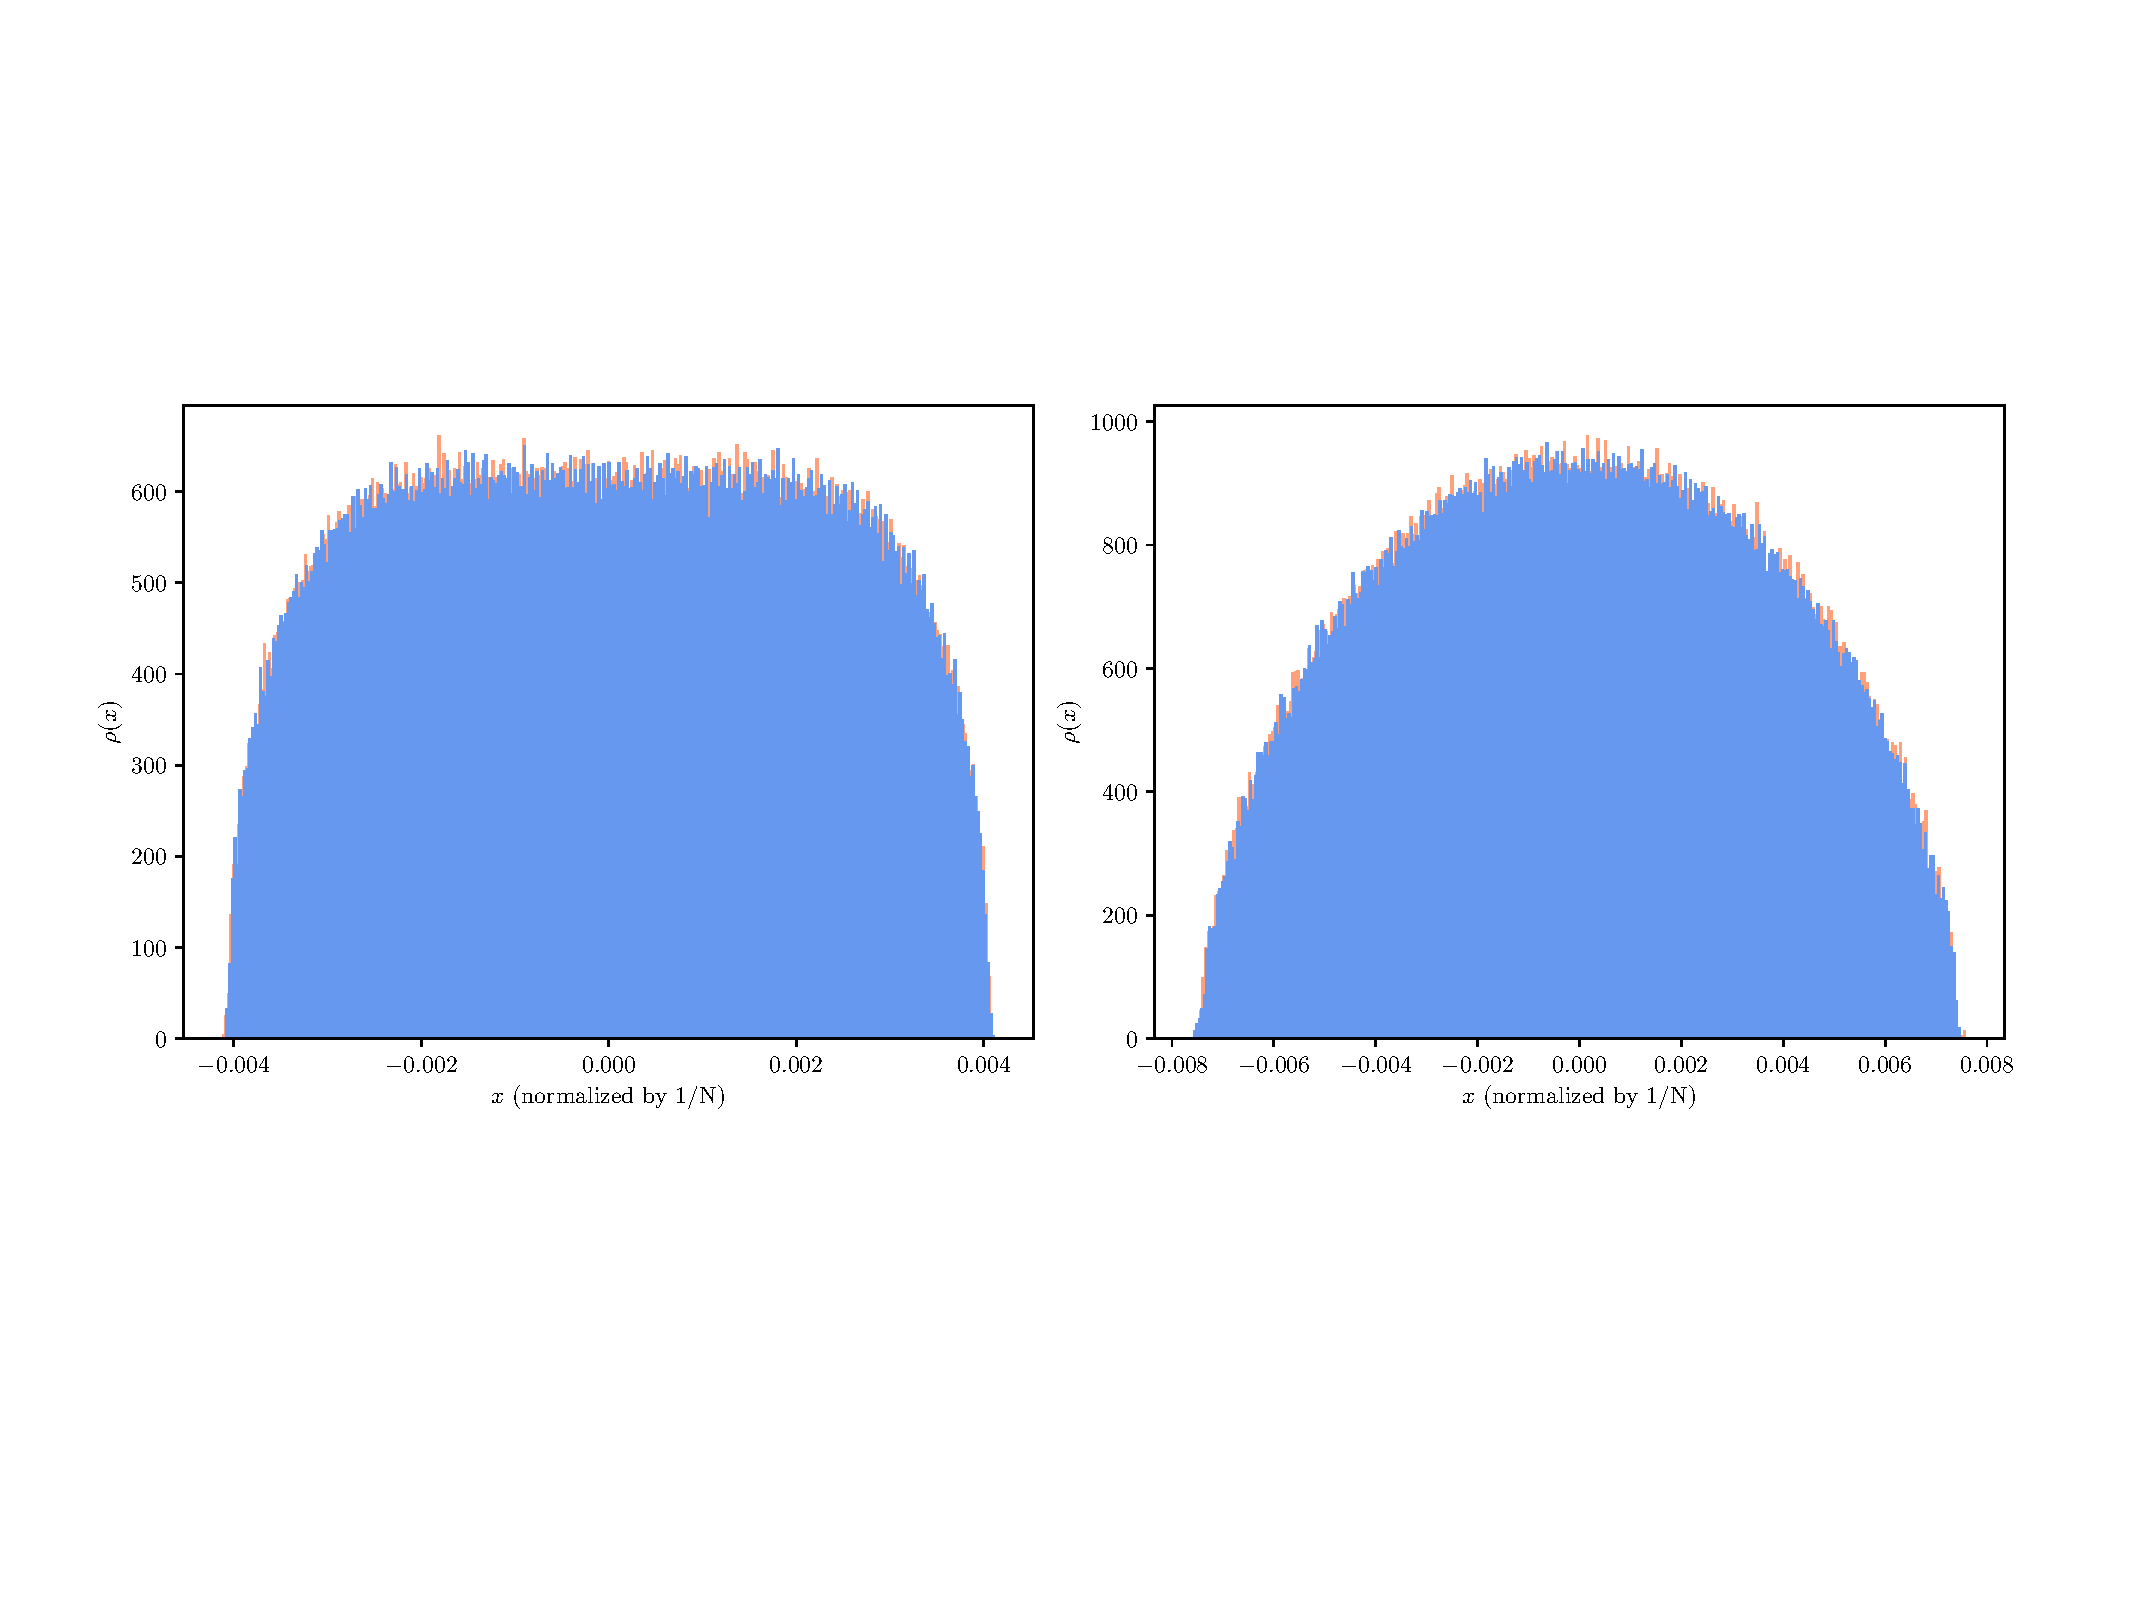
\includegraphics[width=0.95\textwidth]{figs/plot_2MM_evd_both.pdf}
	\caption{\label{fig:2MM_match1}Left: The eigenvalue distribution of two matrices for $g=h=1$ with $N=300$.
	Right: The parabolic distribution for $g = 0, h = -0.04965775$ with $N=300$.}
\end{figure}

We now consider the case where $g=0$ and $h = h_{c}=-0.04965775$, the bootstrap results were not 
very accurate because of slow convergence. We obtained MC results for this case 
and obtain: $t_{2} = 1.1886(15)$ and $t_{4}=2.866(20)$ with $N=300$ after about 4-5 hours of run on a 
laptop. We also explored $h < h_{c}$ and saw that the MC broke down and $t_{4}$ ran away to infinity. 
We show the eigenvalue distribution for this case in the right panel of Fig.~\ref{fig:2MM_match1}. 

It is interesting to consider the same model by flipping the sigs of the quadratic terms in $X,Y$ i.e., 
\begin{equation}
\label{eq:GHM2} 
Z = \int \mathcal{D}X \mathcal{D}Y \exp \Big[-N ~ \mbox{Tr} (-X^2  -Y^2 - h^2 [X,Y]^2 + gX^4 + gY^4) \Big]	
\end{equation} 

\begin{figure}[htbp] 
	\centering 
	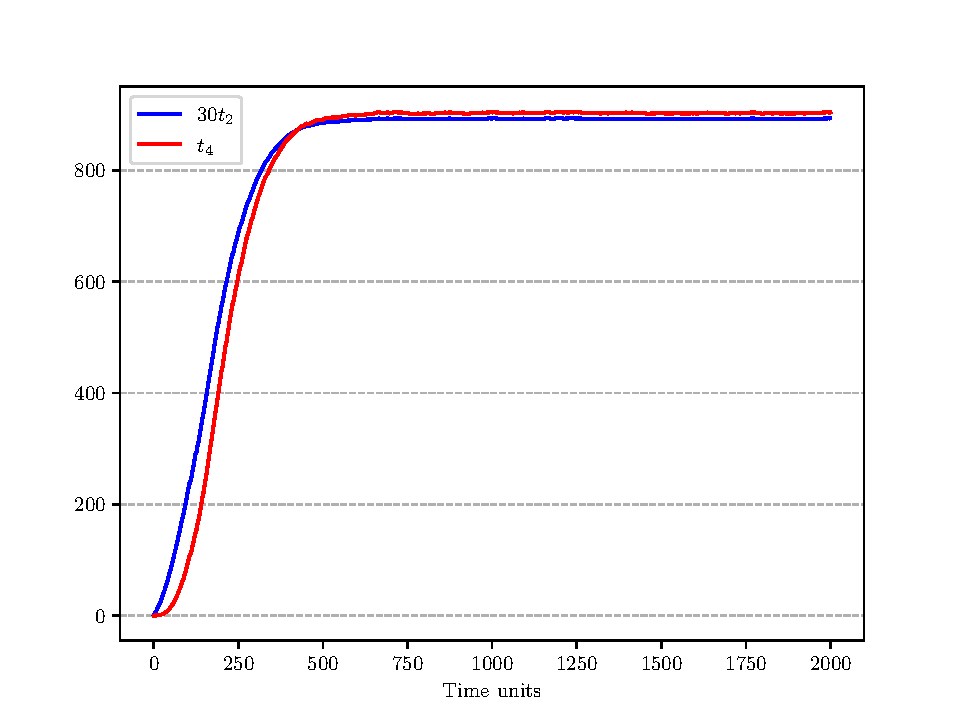
\includegraphics[width=0.75\textwidth]{figs/2MM_symb_t2_t4.pdf}
	\caption{\label{fig:2MM_t2t4}We show $t_{2}$ and $t_{4}$ obtained from MC. 
	The values we obtain for this specific stream of run is: $N=300$ is $t_{2} = 29.73(3)$ and $t_{4} = 903(3)$. 
	This took about 3.5 hours on a laptop since it thermalizes late and we need to run bit longer.}
\end{figure}

\begin{figure}[h] 
	\centering 
	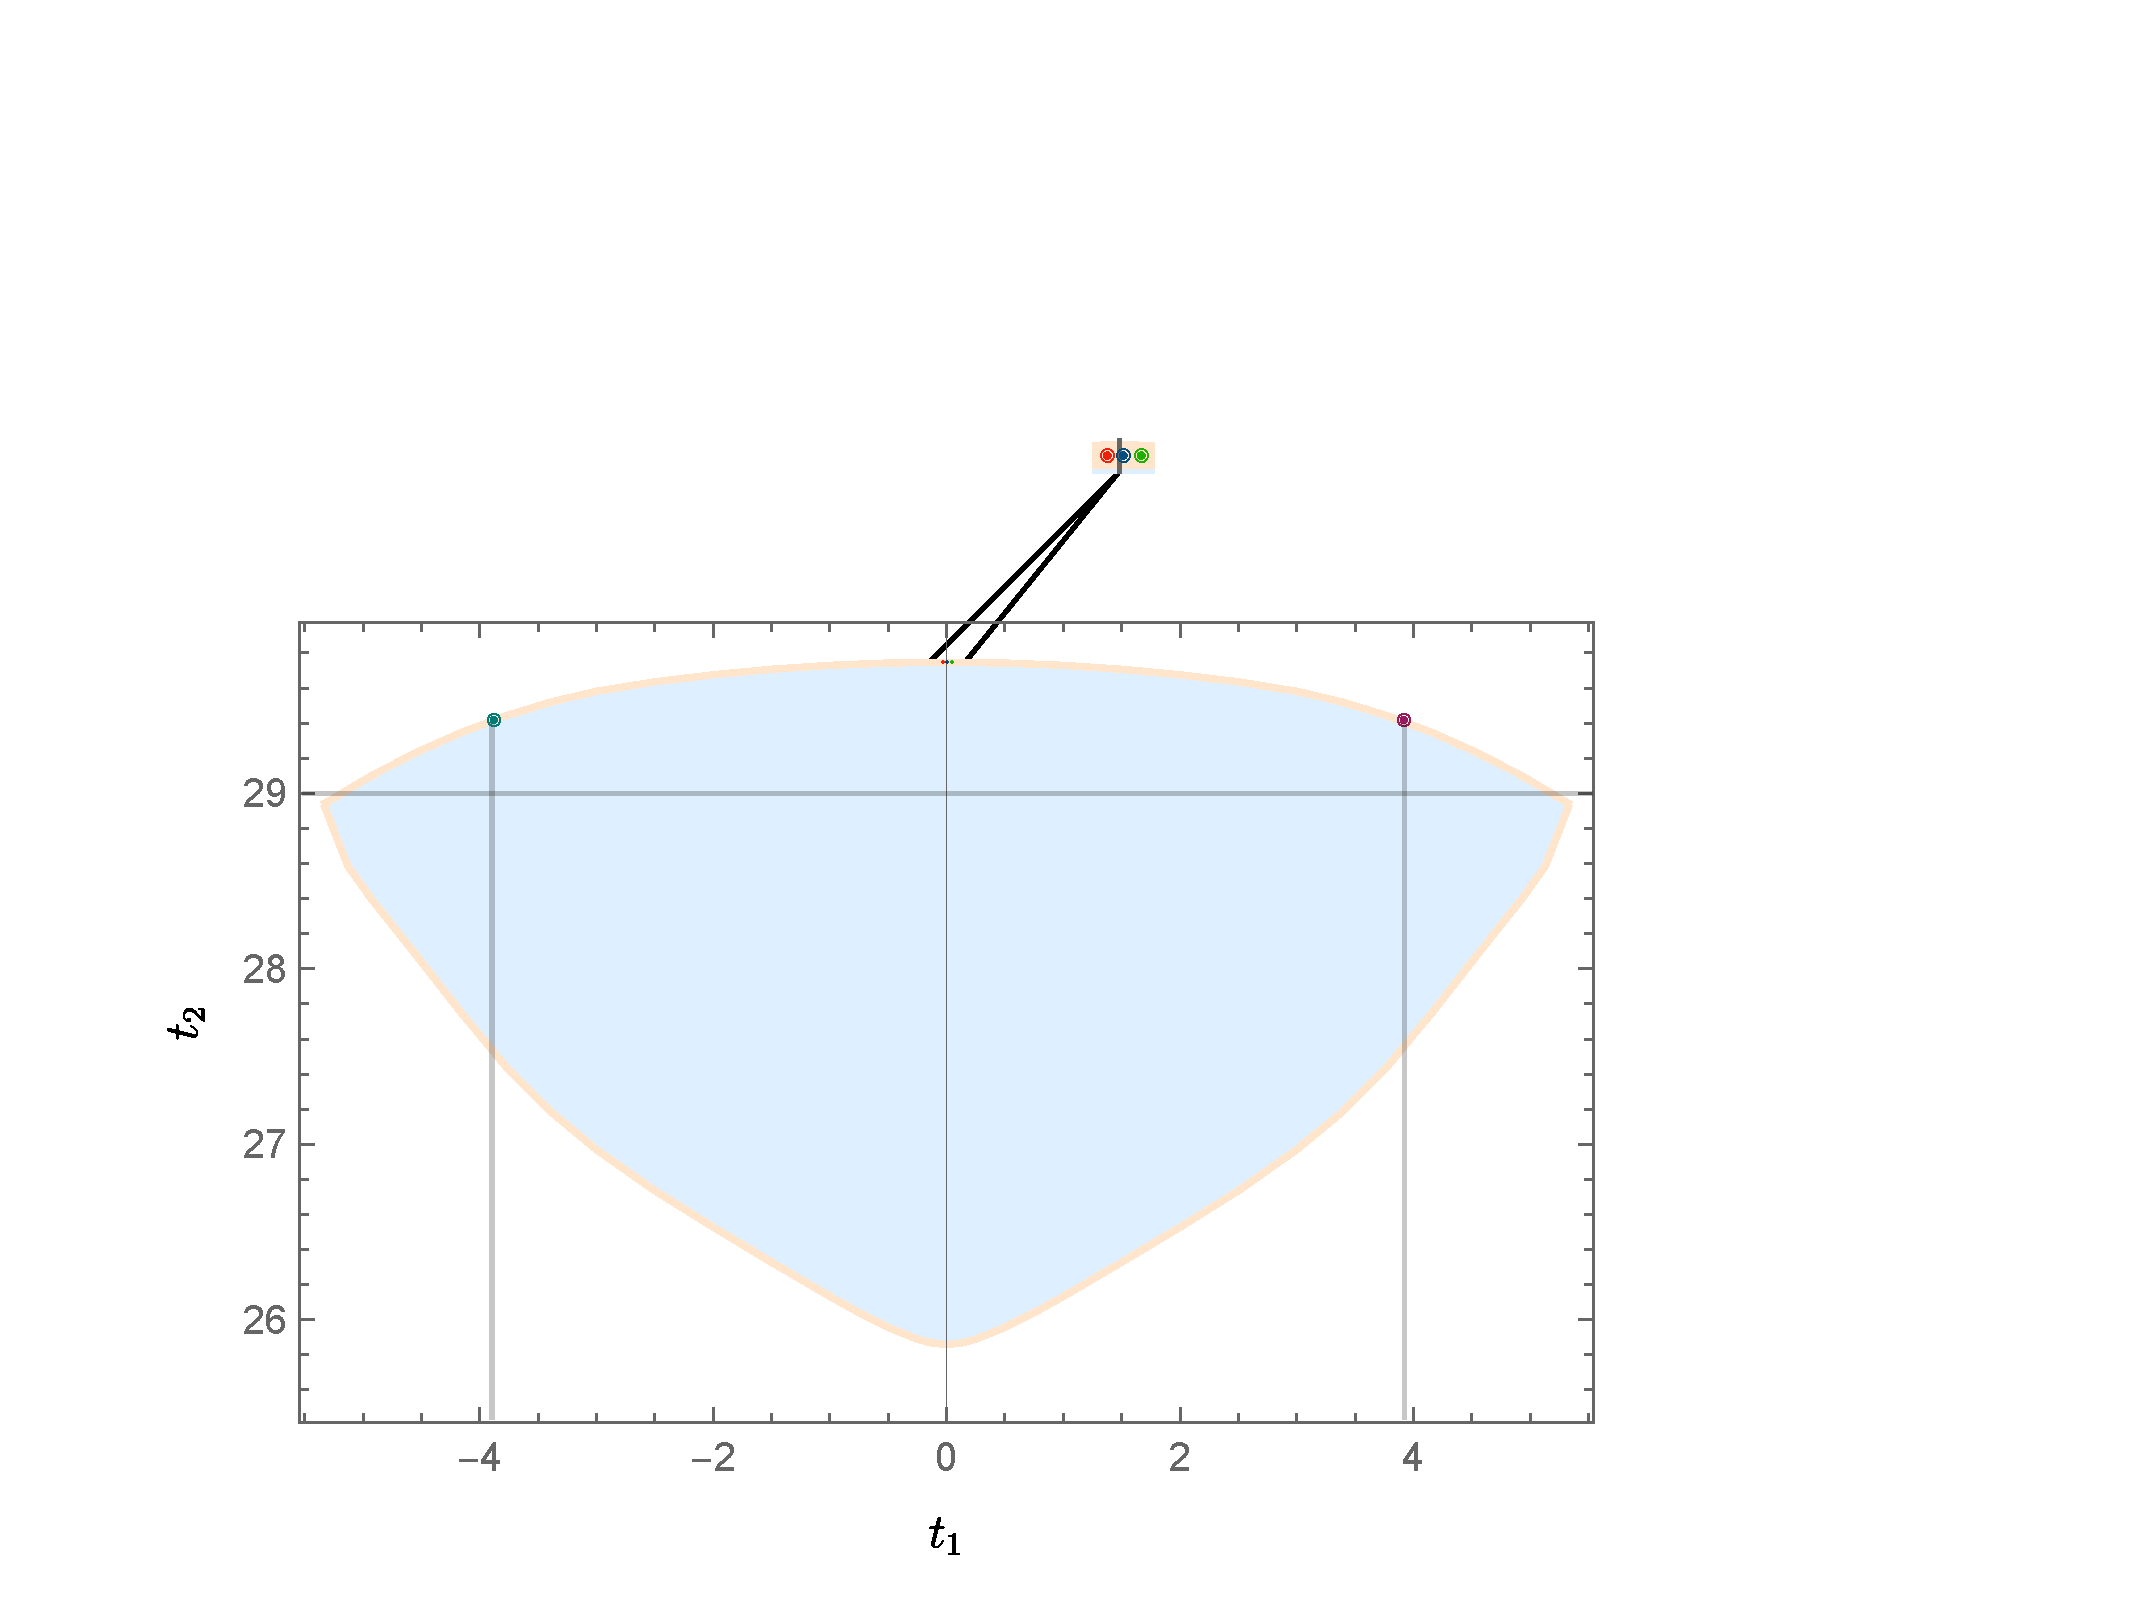
\includegraphics[width=0.75\textwidth]{figs/2MM_symb_ms.pdf}
	\caption{\label{fig:2MM_comp1}We show that the MC results from different streams (different starts) give different results for moments. This is consistent with the region obtained in Ref.~\cite{Kazakov:2021lel} that one will obtain an entire line of solutions. We have shown data from five different MC runs by coloured circles. The three points near $t_{1} \sim 0$ were obtained by starting from a trivial start i.e., ($X,Y = 0$) while the two points with $t_{1} = \pm 3.88(2)$ and $t_{2}=29.41(4)$ were obtained by starting from $X,Y = \mathbb{I}$. 
The figure is used after taking permission from the authors of Ref.~\cite{Kazakov:2021lel}.}
\end{figure}

\begin{figure}[htbp] 
	\centering 
	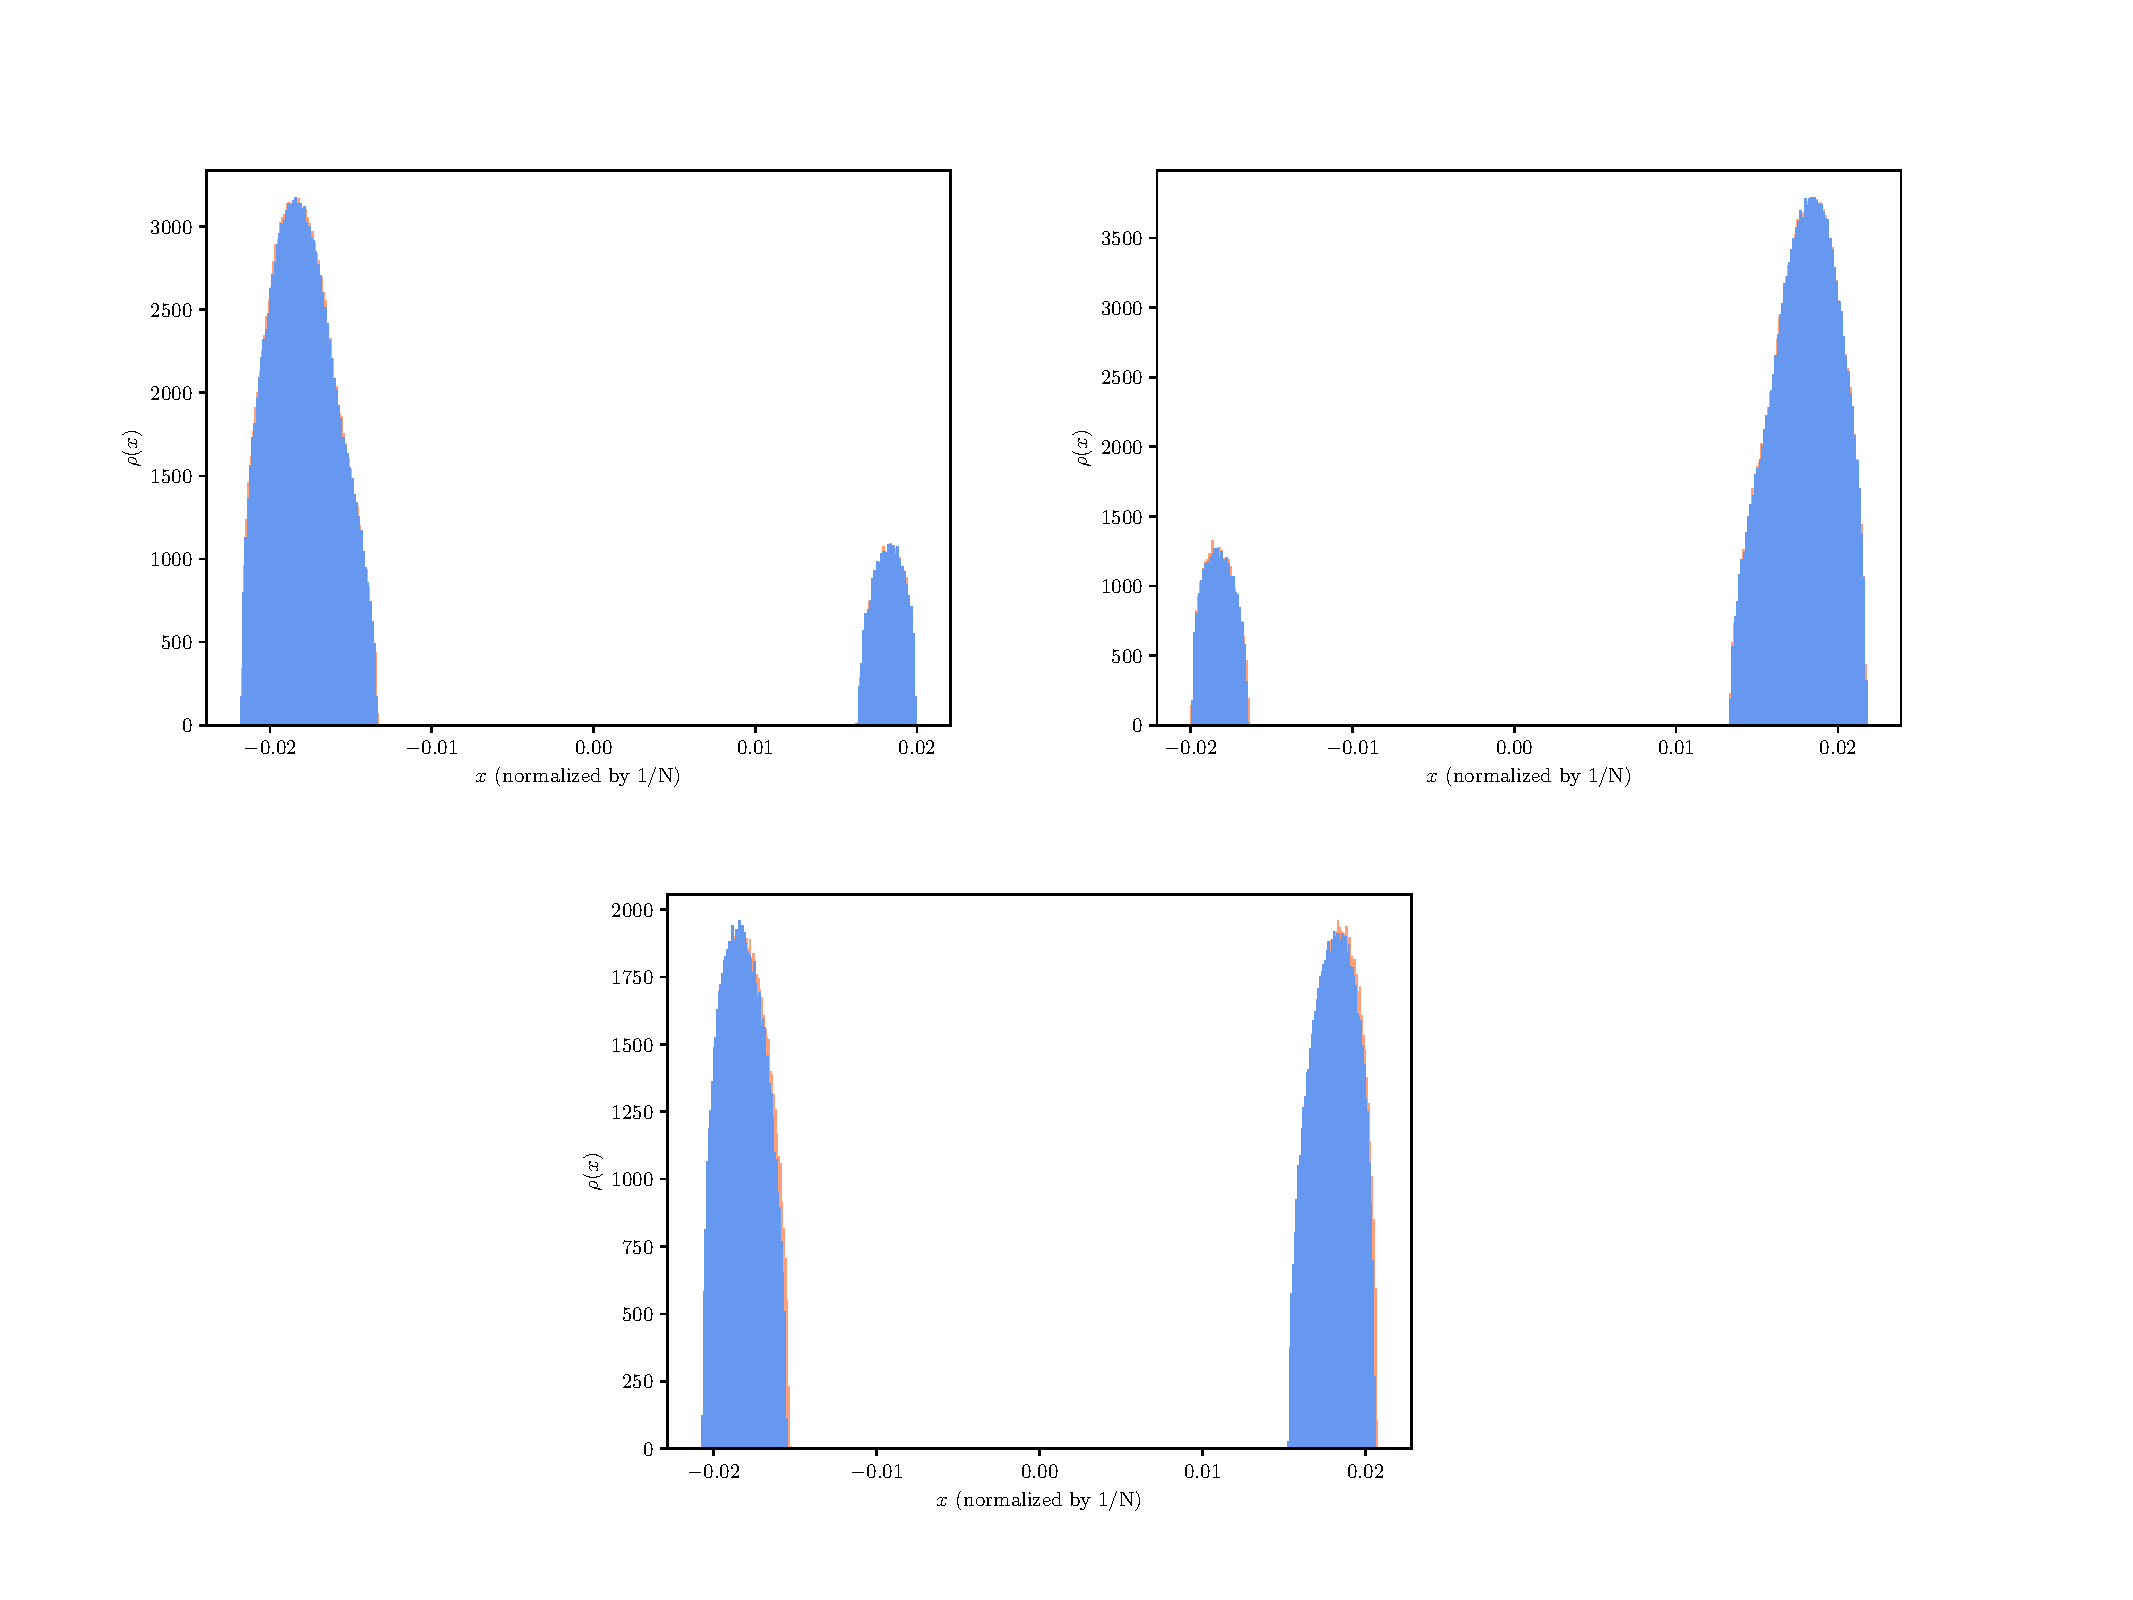
\includegraphics[width=0.85\textwidth]{figs/all_symb_ev.pdf}
	\caption{\label{fig:2MM_evd}The eigenvalue distribution of two matrices for $g=1/30$ and $h=1/15$ 
	with $N=300$ for the potential given in \ref{eq:GHM2} and shown in Fig.~\ref{fig:2MM_comp1}.
	These correspond to green (top left), magenta (top right), red (bottom) data points respectively of Fig.~\ref{fig:2MM_comp1}.
	Note that blue distribution overlaps the orange and means that we have $A \to B$ symmetry as expected.}
\end{figure}

This corresponds to breaking the $\mathbb{Z}_{2}^{\otimes 3}$ symmetry and just keeping the $X \to Y$ part. This results in the $\mathbb{Z}_{2}$ 
symmetry being broken. This model was considered using bootstrap methods in 
Ref.~\cite{Kazakov:2021lel} but compared to the symmetric case, it was tough to get accurate results. 
To benchmark our MC results, we explored this model
with the set of couplings considered in the work above and obtain fairly precise values. 
The results are shown in Fig.~\ref{fig:2MM_comp1}. It is expected that one would be able to
produce entire set of solutions by starting MC from different initial value of matrices. 
%%%%%%%%%%%%%%%%%%%%%%%%%%%%%%%%%
\subsection{\label{subsec:ext_Hoppe}$D$ matrices models with mass term}
After our discussion on models involving one or two matrices, we now turn to matrix models 
with equal or more than three matrices. The model is defined as:
\begin{equation}
\label{eq:HoppeD} 
	Z = \int \mathcal{D}X_1 \cdots \mathcal{D}X_D ~
	\exp\Big[ -Nh\sum_{i}\mbox{Tr}X_{i}^{2} + \frac{N\lambda}{4} \sum_{i < j} \mbox{Tr} [X_i,X_j]^{2}\Big]. 
\end{equation}
If we consider $X_i \mapsto (1+\epsilon) X_i$, it must leave $Z$ invariant, one arrives at the following exact relation: 
\begin{equation}
	D(N^2 -1) = 2 h \langle \mbox{Tr}X_{i}^{2} \rangle 
	- N \lambda \langle \mbox{Tr}[X_i,X_j]^{2} \rangle. 
\end{equation}
This serves as a check of the MC code and is satisfied to a very good accuracy
after ignoring the thermalization cut. We studied this model for $D=3,5$ with 
$h=1, \lambda=4$ and compute: 
\begin{equation}
\label{eq:R2R4} 
	\langle R^2 \rangle =   \frac{1}{DN} \Bigg \langle \mbox{Tr} \sum_{i=1}^{D} X_{i}^2 \bigg \rangle, 
	~~ \langle R^4 \rangle =   \frac{1}{DN} \Bigg \langle \mbox{Tr} \sum_{i=1}^{D} X_{i}^4 \bigg \rangle.  
\end{equation}
The results are given in Table \ref{table:D_YMM_data}. 

\begin{table}[h!]
	\centering
	\begin{tabular}{||c c c||} 
		\hline
		$D$ & $ \langle R^2 \rangle$ & $ \langle R^4 \rangle$ \\ [0.5ex] 
		\hline\hline
		3 & $ 0.279(4) $ & $ 0.158(5) $  \\ 
		5 & $ 0.212(3) $ & $ 0.091(5) $
		 \\ [1ex] 
		\hline 
	\end{tabular}
\caption{The results obtained for $D = 3,5$ matrices models with mass terms are given for $\lambda=4, h=1$ with $N=300$.}
\label{table:D_YMM_data}
\end{table}
Note that it is easy to get the sign of $\mathcal{O}(1/N)$ corrections using Monte Carlo methods.
The simplest way is to do another set of simulation at $N = 100$ and see how $t_{2}$ and 
$t_{4}$ change. It is an interesting problem (in practice) 
to understand how one can apply bootstrap methods 
away from the planar limit where factorization does not hold any more.
\begin{mdframed}[backgroundcolor=blue!3] 
	\textsc{} 
	$\bullet$ Exercise 8: Study the model defined by (\ref{eq:HoppeD}) for $D=3$ by modifying the code given in the appendix for studying the Yang-Mills type model defined by (\ref{eq:CTmodel}). Check that you obtain results consistent
	with that in Table \ref{table:D_YMM_data}.  
\end{mdframed}


%%%%%%%%%%%%%%%%%%%%%%%%%%%%%%%%%
\subsection{\label{subsection:Mchain}Closed and open chain models with $p = 3, 4$}
The matrix chain is a complicated $p$ matrices model which was first considered in \cite{Chadha:1980ri}. We will not mention details of the analytical solution here but instead show the results we obtain for both open and closed versions from numerics later in Fig. \ref{fig:3MM_open}. This model was also studied in context 
of $q$-state Potts model in Refs.~\cite{KAZAKOV198893, KOSTOV1989295, Daul:1994qy}. We define this model in the same way as the original reference: 
\begin{equation}
	\label{eq:Mehta1} 
	Z_{p}(g,c,\kappa) = \int \mathcal{D}M_{1} \cdots  \mathcal{D}M_{p} \exp \mathrm{Tr}\Bigg(\sum_{i=1}^{p} -M_{i}^2  - g M_{i}^{4} + c \sum_{i=1}^{p-1} M_{i}M_{i+1} 
	+ \kappa M_{p}M_{1} \Bigg).
\end{equation} 
Though exact results are available for any $p$ with $\kappa=0$, not much has been explicitly done for $p > 3$ since algebra becomes rather involved. When the chain is connected ($\kappa \neq 0$), the model is \emph{not solvable} with $p \ge 4$. 
\begin{figure}[htbp] 
	\centering 
	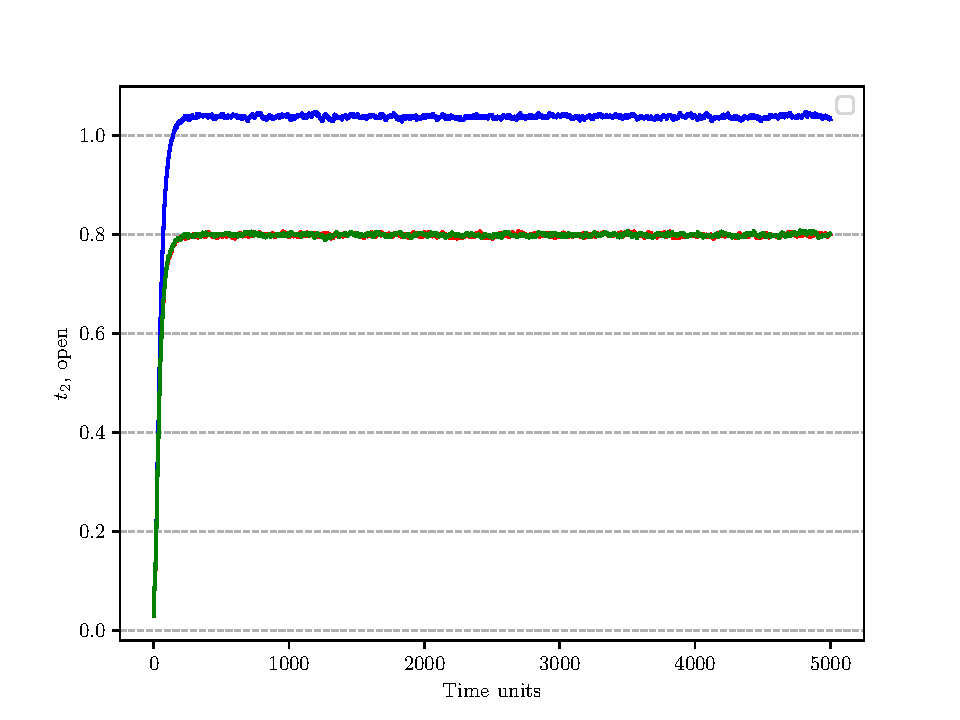
\includegraphics[width=0.75\textwidth]{figs/3MM_open.pdf}
	\caption{\label{fig:3MM_open}We see that two matrices have common $t_{2} = 0.798(3)$ and the third has 
	$t_{2} = 1.037(3)$. This is for $g=1, c=1.35, \kappa=0$ with $N=300$ for the model with three matrices. 
	We have computed errors after discarding the first 1000 time units and using jackknife blocking.}
\end{figure}

\begin{figure}[htbp] 
	\centering 
	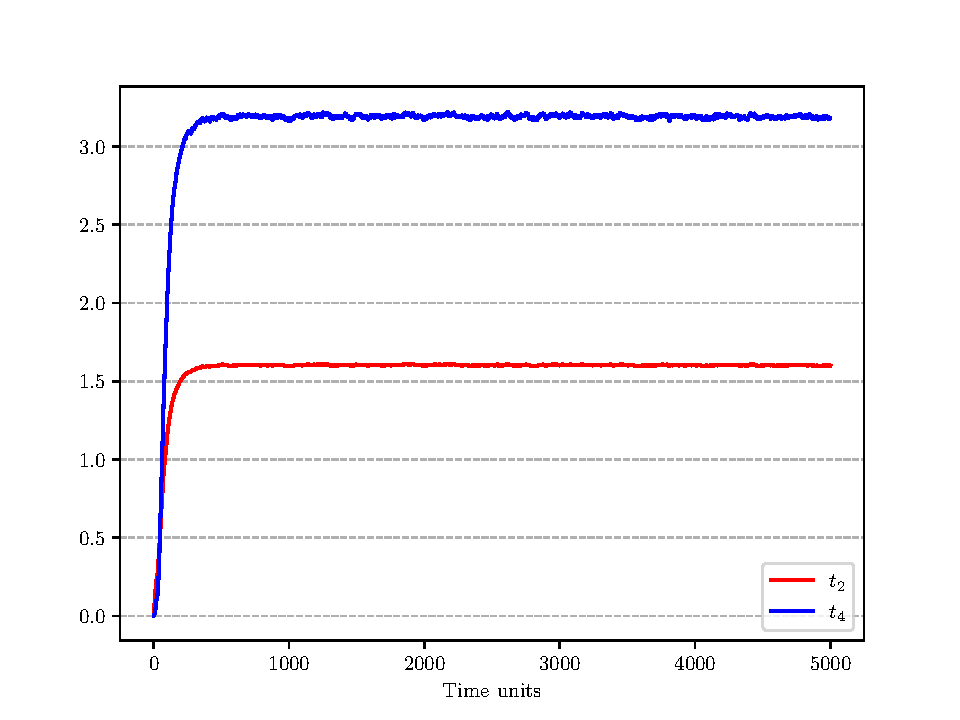
\includegraphics[width=0.75\textwidth]{figs/3MM_closed.pdf}
	\caption{\label{fig:3MM_closed}We find that for closed model with three matrices we find $t_{2} = 1.603(5)$ and $t_{4} = 3.193(5)$. 
	This is for $g=1, c=\kappa=1.35$ for $N=300$. We have computed errors after discarding the first 1000 time units and 
	using jackknife blocking. Note that for this set of parameters it seems like $t_{2} = t_{4}/2$. We found that 
	for $g=2, c=\kappa=1.35$, $t_{2} = 0.775(2)$ and $t_{4} = 0.887(3)$. It is straightforward to understand the behaviour as a function of $g$ at fixed $c, \kappa$ if that is of interest to the reader by using the codes we give.}
\end{figure}
We use Monte Carlo methods to study the open and closed cases of the model with $p = 3,4$ with 
$N = 300$. It would be good if this four matrix model can be \textit{bootstrapped} in the coming years. 
The general $p$ matrix MC code to solve these models 
(well-tested for $p = 3,4$) is available at: 
\begin{center} \texttt{\href{https://github.com/rgjha/MMMC/3\_4\ _MC.py}{https://github.com/rgjha/MMMC/3\_4\_MC.py}} \end{center}

\begin{figure}[htbp] 
	\centering 
	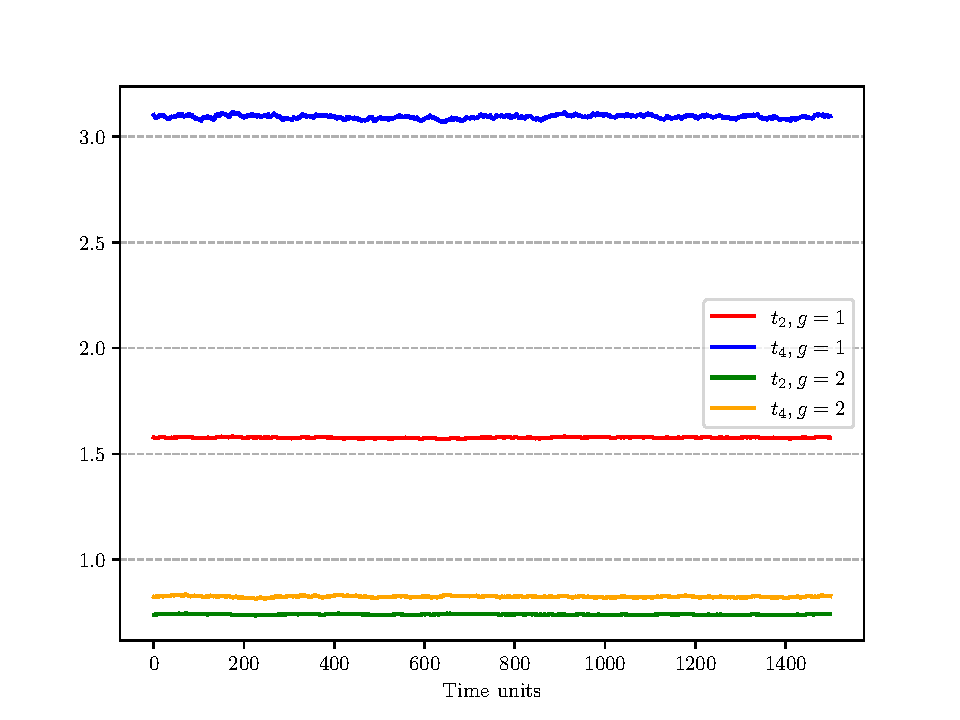
\includegraphics[width=0.75\textwidth]{figs/4MM_g1_g2.pdf}
\caption{\label{fig:4MM_closed1} We show the expectation value for $N=300, c=\kappa=1.35$ with two different $g$. These runs have not started from a \texttt{trivial} start
	as is clear by noting that the traces are non-zero at the first time unit. See Appendix~\ref{sec:BEOC} for details. The data is given in Table~\ref{table:4mchain_data}}
\end{figure}

\begin{table}[h!]
	\centering
	\begin{tabular}{||c c c||} 
		\hline
		$g$ & $ t_2 $ & $t_4 $ \\ [0.5ex] 
		\hline\hline
		1 & $ 1.577(2) $ & $3.093(3)$ \\
		2 & $ 0.741(2)$ & $0.825(3) $  
		\\ [1ex] 
		\hline 
	\end{tabular}
	\caption{The results obtained for closed chain model with four matrices for $g=1,2$ and $N=300, c=\kappa=1.35$.}
	\label{table:4mchain_data}
\end{table}

In order to study the model with four matrices and periodic (closed) boundary conditions 
as defined in (\ref{eq:Mehta1}), we can simply modify the move between $p=3$ and $p=4$ in the codes given by changing $\texttt{NMAT=3}$ to  $\texttt{NMAT=4}$. Note that setting $\kappa=0$ reduces to the open chain case. The broken symmetry correspond to $ c \neq \kappa$ but we have not considered those here. The results for $p=4$ closed symmetric case is given in Table \ref{table:4mchain_data}. 

%%%%%%%%%%%%%%%%%%%%%%%%%%%%%%%%%
\subsection{Multi-matrix Yang-Mills models}
In Sec.~\ref{subsec:ext_Hoppe} we discussed the generalization of Hoppe type matrix models to $D$ matrices
with mass terms. It is also interesting to consider these models without mass terms (i.e., $h=0$) with $D$ matrices. 
We refer to these models as ~`Yang-Mills' type models following Refs.~\cite{Krauth:1998yu,Krauth:1999qw}. 
and point the reader to these for more details. The action is given by: 
\begin{equation}
	\label{eq:CTmodel} 
S = \frac{N}{4\lambda} \int \mbox{Tr} \Bigg( \sum_{i < j}[X_i, X_j]^{2}\Bigg) 
\end{equation}
where $i, j = 1 \cdots D$. The MC code to solve this model is available at:
\begin{center} \texttt{\href{https://github.com/rgjha/MMMC}{https://github.com/rgjha/MMMC}} \end{center}
This model is just the general version of the well-known bosonic part of the IKKT model
where $D=10$. But, this model can be studied for general $D$ and has interesting features, see Ref. \cite{Hotta:1998en}. 
Shortly after the BFSS matrix model\footnote{This matrix model was proposed in Ref.~\cite{Banks:1996vh} by
Banks, Fischler, Shenker, and Susskind. This proposal related the 
uncompactified eleven dimensional $M$-theory in the light cone frame and the 
planar limit of the supersymmetric matrix quantum mechanics describing $D0$-branes. This model has been
well-studied using numerical MC methods~\cite{Catterall:2007fp,Hanada:2008ez,Filev:2015hia,Berkowitz:2016tyy}. 
The publicly available code (by some of the groups) to study these model and its mass deformation (BMN matrix model) and higher-dimensional systems which describes D1/D2 branes~\cite{Catterall:2017lub,Jha:2017zad,Catterall:2020nmn}
is available at \texttt{\href{https://github.com/daschaich/susy}{https://github.com/daschaich/susy}}, while the
highly efficient parallelized code over number of colours for only BFSS and BMN is available at
\texttt{\href{https://sites.google.com/site/hanadamasanori/home/mmmm}
{https://sites.google.com/site/hanadamasanori/home/mmmm}}.
The discussion of these models is not the goal of this article. 
}
was proposed as a description of M-theory, the authors of 
\cite{Ishibashi:1996xs} proposed a reduction of quantum mechanical model down to zero 
dimensions now named after them. This model is related to D-instantons 
in the sense that it has the same action as that of low-energy effective action of D-instantons. 
This model was proposed with the hope to play a key role in description of Type IIB string theory in 
the discrete light cone quantization (DLCQ). Though a complete large $N$ solution of even this model 
is out of reach, there is lot of numerical results are available. 
We also note that there has been some recent work that tries to take the master-field approach to the
IKKT model \cite{Klinkhamer:2021wrv}. This is a promising direction but it is not yet clear how effective 
it is in general. The action for the IKKT model is schematically written as:

\begin{equation}
	\label{eq:IKKT} 
S = \frac{N}{4\lambda} \int \mbox{Tr} \Big( \frac{1}{4} [X_\mu, X_\nu]^{2} + \overline{\psi} \Gamma^{\mu} [A_{\mu},\psi] \Big) 
\end{equation}
where $X_{\mu}$ and $\psi$ are $N \times N$ Hermitian matrices. The gauge field is a ten-dimensional vector and $\psi$ is ten-dimensional Majorana-Weyl spinor field respectively. This model in zero dimensions possesses no usual space-time supersymmetry and is the dimensional reduction of $\mathcal{N}=1$ SYM theory in ten dimensions. 
It is expected that in this model both space and time should be dynamically generated as a result of the dynamics of the large matrices. 
The space-time is expected to emerge entirely from the matrices. 
IKKT model has no free parameters since $\lambda$ can be absorbed in the 
field redefinitions. 

In the original model, since it is a ten-dimensional reduction we have, $\mu, \nu = 1 \cdots 10$. 
It is possible to consider other models where $\mu, \nu = 1 \cdots D$ where $D=4,6$. 
One might worry whether because of the integral measure being over non-compact $X$, 
it is divergent. The convergence issues of the partition function of 
these models for $D=4,6,10$ were studied by Refs.~\cite{Krauth:1998yu,Krauth:1999qw} and 
refer the reader to those for additional details.  
In what follows in these notes, we will ignore the fermionic 
term and only focus on the commutator/bosonic term. 
One of the observables (also known as `size' or i.e., the extent of scalars) 
which we compute in these models is already defined in \ref{eq:R2R4}. 
It is known that $\langle R^2 \rangle$ behaves as $\sqrt{\lambda}$ in the large $N$ limit 
as discussed in Ref.~\cite{Hotta:1998en} but we have not found any previous study
which computes the coefficient. In supersymmetric matrix models like BFSS/BMN, this 
extent of scalars has a dual interpretation in terms of the radius of 
the dual black hole topology.  Our numerical results suggests 
that $ \langle R^2 \rangle = 0.361(2) \sqrt{\lambda}$ 
and $ \langle R^4 \rangle = 0.266(3) \lambda$ with $N = 300$ for a wide range of couplings i.e., 
$\lambda \in [1,100]$. We also note that we see the $\sqrt{\lambda}$ and $\lambda$ behaviour for 
$\langle R^2 \rangle$ and $\langle R^4 \rangle$ valid down to $D=3$. 
One of the standard tests we do for the reliability of the numerical results is 
computing the average action. It can be shown that under a 
change: $X \to e^{\epsilon} X$ if we demand that $Z$ is invariant, 
then we find:
\begin{equation}
\label{eq:SD_IKKT1} 
	\frac{\langle S \rangle}{N^2 - 1} = \frac{D}{4} 
\end{equation}
\begin{figure}[htbp] 
	\centering 
	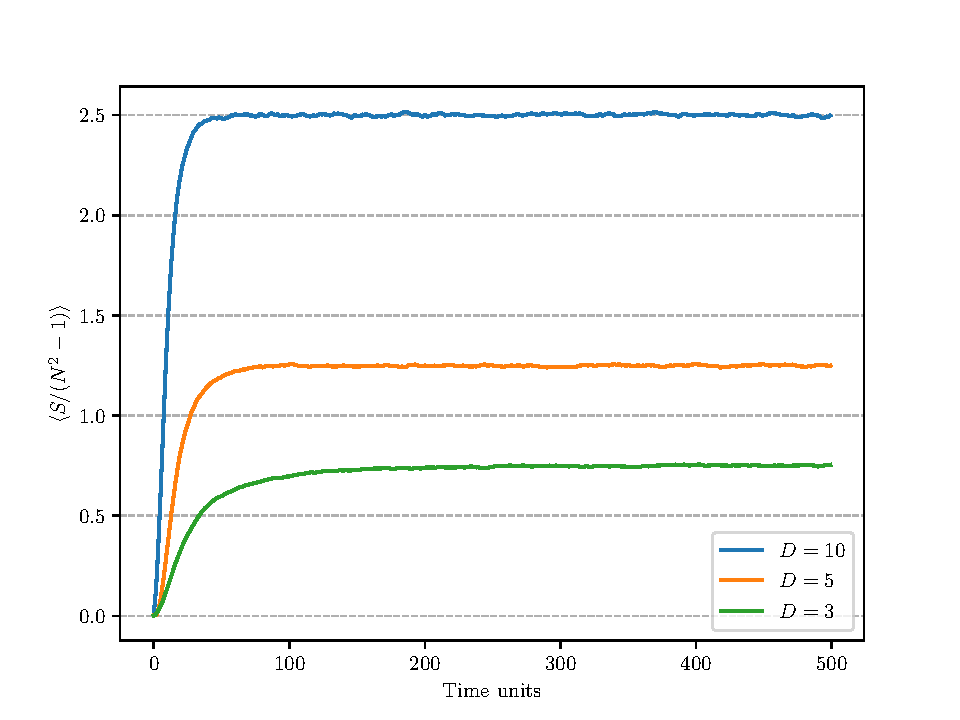
\includegraphics[width=0.75\textwidth]{figs/act_allD_YM.pdf}
	\caption{\label{fig:IKKT_2}The average action (normalized) for the $D=10$ bosonic sector of IKKT model.}
\end{figure}

\begin{mdframed}[backgroundcolor=blue!3] 
	\textsc{} 
	$\bullet$ Exercise 9: Derive (\ref{eq:SD_IKKT1}) by doing the change: $X_{\mu} \mapsto e^{\epsilon}X_{\mu}$ and ignoring 
	$\mathcal{O}(\epsilon^{2})$ terms.
\end{mdframed}

This is an exact result and is used to check the reliability of the simulations. 
We show in Fig. \ref{fig:IKKT_2} that for $D=3,5,10$ we get the correct result and 
hence the \PY~ code above can be fully trusted. The timings for generating 500 time units or trajectories 
with $N=300$ is about \texttt{50000,2300,2000} seconds for $D = 10, 5, 3$ respectively on 
a 2.4 GHz i5 A1989 Mac Pro. The results are collected in Table~\ref{table:D_IKKT_data}. 
\begin{table}[h!]
	\centering
	\begin{tabular}{||c c c||} 
		\hline
		$D$ & $ \langle R^2 \rangle$ & $ \langle R^4 \rangle$ \\ [0.5ex] 
		\hline\hline
		3 & $1.129(3) $ & $2.71(2) $  \\ 
		5 & $0.608(2) $ & $0.765(3) $  \\
		10 & $0.361(2)$ & $0.266(3)$
		 \\ [1ex] 
		\hline 
	\end{tabular}
\caption{The results obtained for various $D$ YM matrix models are given for $\lambda=1$ with $N=300$.}
\label{table:D_IKKT_data}
\end{table}

\begin{mdframed}[backgroundcolor=blue!3] 
	\textsc{} 
	$\bullet$ Exercise 10: Carry out the MC computation for the bosonic Yang-Mills type matrix model with $D=6$. After sufficient thermalization cut, check that the results for average action is consistent with exact result obtained using Schwinger-Dyson equations within errors. Refer to appendix for the \PY~ code and to perform jackknife error analysis with sufficiently large block size. Compute the ratio $\langle R^4 \rangle / \langle R^2 \rangle$ for fixed $\lambda=1$. 
\end{mdframed} 


%%%%%%%%%%%%%%%%%%%%%%%%
\section{Summary}
In these notes, we have considered wide range of matrix models starting from the simplest one matrix Hermitian matrix model and then considering models with two/three matrices and then Yang-Mills type models with up to ten matrices. We described the Monte Carlo method 
to numerically study them in the large $N$ limit. We obtained some new results and confirmed several known results from analytical methods and recently developed bootstrap program. We hope this introduction will encourage interested readers 
to carry out these numerical computations using the programs provided and will eventually lead to new ways of solving matrix models and to bootstrap the models not yet explored.
 
%%%%%%%%%%%%%%%%%%%%%%%%

\vspace{8mm}

\subsection*{Acknowledgements}
The author is indebted to Pedro Vieira
for discussions and encouragement. We thank Vladimir Kazakov 
and Zechuan Zheng for helpful email correspondence and for 
permission to use a figure from their paper. The author is supported by a 
postdoctoral fellowship at the Perimeter Institute for Theoretical Physics. Research at Perimeter 
Institute is supported in part by the Government of Canada through the Department of Innovation, 
Science and Economic Development Canada and by the Province of Ontario through 
the Ministry of Economic Development, Job Creation and Trade.
The author would like to acknowledge support in the past from 
the Department of Science \& Technology, Government of India's KVPY
(Kishore Vaigyanik Protsahan Yojana) Scholarship during 2008-2010, 
the European Union for Erasmus Mundus (Lot 13) scholarship during 2010-2011, 
and the Department of Physics at Syracuse University for research and teaching
assistantship during 2013-2019. 
% Though I would also like to thank Sci Hub in acknowledgements, some might not like it! 
%%%%%%%%%%%%%%%%%%%%%%%%



%%%% Appendices now %%%%
%\newpage
\vspace{16mm}
\appendix
\begin{center} \large{\textsc{Appendices}}\end{center}
\section{\label{sec:Ortho_pol1}Orthogonal polynomials}
One of the methods we discussed for the solution of 
large $N$ limit of matrix models was the saddle point approximation. 
However, this method is not useful 
to understand the terms subleading in $1/N$. The method 
of orthogonal polynomials introduced by Bessis et al. in Ref.~\cite{Bessis:1980ss} 
is usually used for such computations. In fact, it is also very useful in 
solving two matrix 
models. These polynomials are defined as:
\begin{equation}
	\label{eq:ortho_nn} 
	\int d\lambda e^{-V(\lambda)} P_{n}(\lambda)
	P_{m}(\lambda) = \int d \mu(\lambda) P_{n}(\lambda)
	P_{m}(\lambda) = a_{n} \delta_{mn} 
\end{equation}
where $d \mu(\lambda) = d\lambda e^{-V(\lambda)}$ is the measure. 
The basic idea is to rewrite the Vandermonde determinant appearing after we change from matrix basis to the basis of eigenvalues. 
\begin{equation}
	\Delta(\lambda) = \det(\lambda_{i}^{j-1})_{1 \le i, j \le N} = \det(P_{j-1}(\lambda_i))_{1 \le i, j \le N}
\end{equation}
These polynomials can solve:
\begin{equation}
	\label{eq:mm_main}
	Z = \int dM \exp[-\mbox{Tr} V(M)] 
\end{equation}
In fact, it can be shown that \ref{eq:mm_main} is equivalent to:
\begin{equation}
\label{eq:ZOP} 
	Z = N! ~ a_{0}^{N} \prod_{k=1}^{N-1} f_{k}^{N-k}
\end{equation}
where $f_{k} := a_{k}/a_{k-1}$. Hence, solving the matrix model is now equivalent to solving for the 
normalization appearing in \ref{eq:ortho_nn}. As we have shown in Sec.~\ref{sec:MMAres}, 
this method was used to solve the unitary 
matrix model. In fact, this method was also used to study the Ising Model on a random graph as two-matrix model 
\cite{Kazakov:1986hu}
and the partition function is given by:
\begin{equation}
	\label{eq:Kaz1} 
	Z = \int \mathcal{D}A \mathcal{D}B \exp N \mbox{Tr} \Bigg(-A^2 -B^2 + 2c AB -g \frac{A^3}{3} - g\frac{B^3}{3}  \Bigg)
\end{equation}
Note that this has a $\mathbb{Z}_{2}$ symmetry because of 
the partition function being invariant under $A \mapsto B$. This is however broken in finite magnetic field ($h \neq 0$) as clear from the partition fuction below:

\begin{equation}
	\label{eq:RIsing1} 
	Z = \int \mathcal{D}A \mathcal{D}B \exp N \mbox{Tr} \Bigg(-A^2 -B^2 + 2c AB -g_{A}e^{h} \frac{A^3}{3} 
	- g_{B}e^{-h} \frac{B^3}{3}  \Bigg)
\end{equation}

After the solution of Ising model on random graph, this was extended to admit magnetic fields
\cite{Boulatov:1986sb} as well. We will not discuss the entire solution but will 
sketch the solution. In this paper, the authors also computed the critical exponents 
and found different results than Onsager's case for regular square lattice. 
The exponents satisfied the usual Rushbrooke's law ($\alpha + 2\beta+\gamma=2$) 
and Widom's scaling law: $\gamma/\beta = \delta -1$. 
These values coincide with the  exponents obtained in a three-dimensional spherical model. 
This is a striking correspondence between exponents of two different models in different dimensions! 
In fact, after few years, while discussing the Yang-Lee edge sigularity (YLES) on dyamical graph, 
it was shown that an additional exponent $\sigma =1/2$ 
also behaved accordingly. 
We have listed the exponents in Table (\ref{table:crit_exp}) for the curiosity of the reader.
\begin{table} 
	\begin{center} 
\begin{tabular}{|c|c|c|}
	\hline Crit. exponents & Ising model on random planar graph & Ising model on regular lattice \\
	\hline$\alpha$ & $-1$ & 0 \\
	$\beta$ & 1/2 & 1/8 \\
	$\gamma$ & 2 & 7/4 \\
	$\delta$ & 5 & 15 \\
	$\nu d$ & 3 & 2 \\
	$\gamma_{\text {str}}$ & -1/3 & - \\
	\hline
\end{tabular}
\end{center} 
	\caption{Summary of critical exponents obtained for two-dimensional Ising model on different graphs} 
	\label{table:crit_exp}
	\end{table} 
By turning the partition function in terms of eigenvalues, we get:
\begin{equation}
	Z = \int dX dY \Delta(X) \Delta(Y)
	 \exp \Big[-N \sum_{i} (x_{i}^2 + y_{i}^{2} +2c x_{i}y_{i} + 4ge^{h}x_{i}^{4} + 4ge^{-h}y_{i}^4) \Big]
	\end{equation}
It is now clear that we would need two polynomials $P_{k}(x)$ and $Q_{j}(y)$ for this case 
such that their determinant matches $\Delta(X)$ and $\Delta(Y)$ respectively. 
These polynomials satisfy the following orthonormal condition: 
\begin{equation}
\int dx dy e^{-N V(x,y)} P_{k}(x) Q_{j}(y) = h_{k} \delta_{kj}
\end{equation}
They also satisfy several recursion relations for which the interested reader can refer to 
\cite{Boulatov:1986sb}:

\begin{equation}
	Z = \int dX dY \det[P_{r}(x_k)] \det[Q_{r}(y_k)] \exp\Big[-N \sum V(X,Y)\Big]
\end{equation}
where we have denoted $\sum_{i} (x_{i}^2 + y_{i}^{2} +2c x_{i}y_{i} + 4ge^{h}x_{i}^{4} + 4ge^{-h}y_{i}^4)$ by $V(X,Y)$. 
Transforming to the eigenvalue basis of both matrices $X$ and $Y$ and using the expansion of the determinant we get:

\begin{align}
	Z &= \epsilon^{i_1 \cdots i_N} \epsilon^{j_1 \cdots j_N} \int dx_{1 \cdots N}
	dy_{1 \cdots N} P_{i_{1}}(x_1) \cdots P_{i_{N}}(x_N)
	Q_{j_{1}}(y_1) \cdots Q_{j_{N}}(y_N)
	e^{-N \sum V(x_i,y_i)} \nonumber  \\  
	&= \epsilon^{i_1 \cdots i_N} \epsilon^{j_1 \cdots j_N} \prod_{r=1}^{N} \int dx_{r} dy_{r} e^{-N V(x_r, y_r)} P_{i_r}(x_r) Q_{j_r}(y_r) \nonumber  \\  
	&=  N! \prod_{i=0}^{N-1} h_{i} 
	\label{eq:ising_r2}
\end{align}
We can define $f_{k} := h_k/h_{k-1}$ and hence 
(\ref{eq:ising_r2}) implies:

\begin{equation}
	\log Z_{N}(c,g,h) = \log N! + N \log h_0 + \sum_{k=1}^{N-1} (N-k) \log f_{k} 
\end{equation}
One is usually interested in computing the quantity (the subscript `pc' denotes planar/continuum limit i.e., $ N \to \infty$):
\begin{equation}
	F_{pc} = \frac{1}{N^2} \log\Bigg( \frac{Z(c,g,h)}{Z(c,0,0)}\Bigg) = \frac{1}{N} \sum_{k=1}^{N-1} \left(1 - \frac{k}{N} \log \Big(\frac{f_k}{f_{k,0}}\Big)\right)
\end{equation}

\section{\label{sec:math_code}\MA~code for the solution of one-matrix model}
We now give the details to solve the one matrix model in \MA. For this we consider the potential:
\[ V(Y) = \frac{Y^2}{2} + \frac{gY^4}{4}.\]
As we have shown in the text, for this case, the higher moments of the trace of $Y$ are related and hence we will just calculate $\mbox{Tr}~Y^2$ in the planar limit (normalized by $N$). We give the code below for computing $t_{2}$ with $g=1$. The reader is encouraged to try and change $g$ and see how the results change.

\begin{mdframed}[backgroundcolor=magenta!3] 
	\begin{footnotesize} 
		\noindent 
		\verb"V[y_]=y^2/2+(g y^4)/4;"\\
		\verb"G[x_]=Integrate[-1/(2\[Pi]I)Sqrt[x^2-a^2]/Sqrt[y^2-a^2](N V'[y])/(x-y),{y,-a,a}," \newline
		\verb"Assumptions->{x>a,a>0}];"\\
		\verb"sol=Series[G[x],{x, \[Infinity], 1}]-N/x//Simplify//Solve[# == 0,a]&//Simplify; "\\
		\verb"Series[G[x],{x,\[Infinity], 5}]//Normal; "\\
		\verb"{Coefficient["\%\verb", x, -3]}/N;"\\
		\%\verb" /. sol;"\\
		\%\verb"/.{g -> 1}//Chop//N// Grid"
	\end{footnotesize} 
\end{mdframed}

%%%%%%%%%%%%%%%%%%%%%%%%%%%%
\section{\label{sec:BEOC}Brief explanation and comments on 
running the \PY~code}
We provide programs which can deal with several different types of Hermitian matrix models. The instructions on how to use them can be found at:  
\begin{center} \texttt{\href{https://github.com/rgjha/MMMC\#readme}{https://github.com/rgjha/MMMC}} \end{center}
 The list of all programs are summarized below:
\begin{enumerate}
	\item One matrix model: \texttt{\href{https://github.com/rgjha/MMMC/1MM.py}{https://github.com/rgjha/MMMC/1MM.py}}
	\item Two matrix Hoppe-type models: \texttt{\href{https://github.com/rgjha/MMMC/2MM.py}{https://github.com/rgjha/MMMC/2MM.py}}  
	\item $p=3,4$ matrix chain models: \texttt{\href{https://github.com/rgjha/MMMC/MMC_3_4.py}{https://github.com/rgjha/MMMC/MMC\_3\_4.py}}
	\item Yang-Mills type models: \texttt{\href{https://github.com/rgjha/MMMC/YM_type.py}{https://github.com/rgjha/MMMC/YM\_type.py}}
\end{enumerate}
In addition to this, we also give codes for one matrix model and $D$ matrices Yang-Mills models in Appendix~\ref{sec:1MMPYC}, and \ref{sec:YMC} respectively.
These codes can also be modified to other potentials as required. In general, only two routines need modifications. 
One is $\texttt{def potential(X)}$ and other is the $\texttt{def force(X)}$. 
The first involves (mostly) trace of product of matrices and the second is the 
derivative of those matrix traces. 
These codes in \PY~is rather terse
and are all under $\texttt{300}$ lines each
while about $\sim 85\%$ of them are common parts like:
leapfrog integrator, Metropolis step, saving/reading configuration file, 
and plotting the data. We have tried no optimization to make it efficient and the
only motivation is that someone who has never ran a MC code can do
so quickly and use it as guidance for deriving exact results or for
bootstrapping purposes. We need to take care of few things which are 
mentioned below.  

\begin{itemize} 
\item The acceptance rate should always be more than $50\%$
on average. If the acceptance rate is less than this, we
must reduce the size of leapfrog integrator by reducing 
$\texttt{dt}$ in the global definitions at the starting. Note that 
reducing this time step makes the computation more expensive. 
This time step needs to be modified accordingly if you want to explore values of $N$
more than $N = 300$ which we mostly restrict to in these notes. The code will give a warning
if the acceptance falls below $50\%$.  
\item We must not change the step size during the entire time of simulation. It has to be 
chosen to a value where acceptance is reasonable and then kept constant. If the acceptance
doesn't improve eve after reducing the time step, it signals an error in the force term.
\item As a thumb rule, during the evolution, the $\texttt{delta H}$ (which is the sum of
trace of potential (or action) and momenta) should fluctuate around zero
with both negative and positive signs. However, this might not be true from the start, and should
be monitored after sufficient thermalization. After thermalization, we should have 
$\langle e^{-\Delta H} \rangle = 1$ within errors. You can see why this is true in the section on 
solution to the selected exercises. 
\item We usually start a run by setting all matrices to zero (also referred here as \texttt{fresh} or 
\texttt{trivial} start). Then as the evolution progresses, we store a new configuration by rewriting older one
every 10 time units. The configuration file stores $N \times N$ matrices over which we do the matrix integral 
in binary format as a \texttt{numpy array}. 
The size of this file can vary from few MB up to 50 MB or more depending on 
$\texttt{NMAT}$ and $\texttt{NC}$. If you are not doing the run for the first time, 
it is better if you read in the configuration file as this will be more efficient.  
Note that this can only be done if $\texttt{NMAT}$ and $\texttt{NC}$ are the same or else
it will throw some error. This can be modified easily to suit user's requirements. 
\item The code produces output files with name starting with $\texttt{t2*.txt}$ and $\texttt{t4*.txt}$
which are moments of the matrices. The number of columns in these files will be equal to 
number of different matrices you considered in the potential i.e., $\texttt{NMAT}$. 
If you consider a ten matrix model (maximum we have used in these notes),
these files will have ten corresponding columns. 
\item It is common practice among those who use Monte Carlo to never measure an 
observable every time unit (because of autocorrelation), but for these simple models, it is probably okay to do so. However, if you
have enough computer time and want to do a systematic study, you should increase it. This is controlled by \texttt{GAP}. Another way to make sure that this is accepted for is to use a sufficiently large block size when computing errors using jackknife method. 
\item Note that Monte Carlo is a sampling method and hence we will always have errors for the expectation values. The errors must be carefully computed using either jackknife binning or some other method. 
\end{itemize} 
Though these codes have been checked several times over 
and compared to known solutions (where available), it is possible 
that there might still be minor bugs in them. If you encounter a problem or have questions, please contact the author. 


%%%%%%%%%%%%%%%%%%%%
\vspace{18mm}
\section{\label{sec:1MMPYC}\PY~code for Hermitian one matrix model}
We provide the code in this section to study the 1MM using the Monte Carlo method. By running the code given below
on a modern laptop, we get the result shown in 
Fig. \ref{fig:1MM_res}. We can readily extend this code (by changing $\texttt{NMAT}$) to study matrix models where the integration is over several different matrices. 
To run this code using Mac/Linux system (assuming you have \PY~installed) just type in terminal: 
$\texttt{python 1MM\_MC.py 0 1 300 200}$. The code takes four input arguments. The first two are binary arguments
related to whether we are reading any old configuration file and whether we want to save the one which will be 
generated. $\texttt{0 1}$ means that we are not reading any configuration but we want to save it for later use. 
The third argument is the size of the matrices to consider, in an ideal world, planar limit is $ N \to \infty$ but here
we have $\texttt{N = 300}$. The last argument is the 
number of trajectories we want to run the simulation. 
To converge to the correct answer $\texttt{500}$ should be enough but to accurately 
get to third or four decimal place of accuracy, 
more than $\texttt{5000}$ may be needed. 
It takes about 35-40 minutes to run 500 time units 
with $\texttt{N = 300}$ on a modern laptop. 


\begin{footnotesize} 
\begin{mdframed}[backgroundcolor=mauve!3] 
\begin{lstlisting}[language=Python]
#!/usr/bin/python3
# -*- coding: utf-8 -*-
import time 
import datetime 
import sys
import numpy as np
import random
import math
from numpy import linalg as LA
from matplotlib.pyplot import *
from matplotlib import pyplot as plt

startTime = time.time()
print ("STARTED:" , datetime.datetime.now().strftime("%d %B %Y, %H:%M:%S"))
if len(sys.argv) < 5:
  print("Usage:python",str(sys.argv[0]),"READ-IN? " "SAVE-or-NOT? " "NCOL " "NITERS")
  sys.exit(1)

READIN = int(sys.argv[1])
SAVE = int(sys.argv[2])
NCOL = int(sys.argv[3]) 
Niters_sim = int(sys.argv[4])

if Niters_sim%GAP != 0:
  print("'Niters_sim' mod 'GAP' is not zero ")
  sys.exit(1) 

NMAT = 1
g = 1.0
dt = 1e-3
nsteps = int(0.5/dt) 
GAP = 2.
cut = int(0.25*Niters_sim) 
X = np.zeros((NMAT, NCOL, NCOL), dtype=complex)
mom_X = np.zeros((NMAT, NCOL, NCOL), dtype=complex)
f_X = np.zeros((NMAT, NCOL, NCOL), dtype=complex)
X_bak = np.zeros((NMAT, NCOL, NCOL), dtype=complex)
HAM, expDH, trX2, trX4, MOM = [], [], [], [], []
t2_ex = [None] * NMAT
t4_ex = [None] * NMAT

print ("Matrix integral simulation of%2.0f MM"%(NMAT)) 
print ("NCOL =" " %3.0f " ","  " and g =" " %4.2f" % (NCOL, g)) 
print ("------------------------------------------------------")

def dagger(a):
    return np.transpose(a).conj()

def box_muller():  
    PI = 2.0*math.asin(1.0);    
    r = random.uniform(0,1)
    s = random.uniform(0,1)
    p = np.sqrt(-2.0*np.log(r)) * math.sin(2.0*PI*s)
    q = np.sqrt(-2.0*np.log(r)) * math.cos(2.0*PI*s)
    return p,q

def copy_fields(b):
    for j in range(NMAT):
        X_bak[j] = b[j]
    return X_bak

def rejected_go_back_old_fields(a):
    for j in range(NMAT):
        X[j] = a[j]
    return X

def refresh_mom():
    for j in range (NMAT):
        mom_X[j] = random_hermitian()
    return mom_X

def random_hermitian():
    tmp = np.zeros((NCOL, NCOL), dtype=complex)
    for i in range (NCOL):
        for j in range (i+1, NCOL):
            r1, r2 = box_muller()
            tmp[i][j] = complex(r1, r2)/math.sqrt(2)
            tmp[j][i] = complex(r1, -r2)/math.sqrt(2)
    for i in range (NCOL):
        r1, r2 = box_muller()
        tmp[i][i] = complex(r1, 0.0) 
    return tmp


def makeH(tmp):
    tmp2 = 0.50*(tmp+dagger(tmp)) - (0.50*np.trace(tmp+dagger(tmp))*np.eye(NCOL))/NCOL
    for i in range (NCOL):
        tmp2[i][i] = complex(tmp[i][i].real,0.0)  
    if np.allclose(tmp2, dagger(tmp2)) == False:
        print ("WARNING: Couldn't make hermitian")
    return tmp2


def hamil(X,mom_X):
    ham = potential(X) 
    for j in range (NMAT):
        ham += 0.50 * np.trace(np.dot(mom_X[j],mom_X[j])).real 
    return ham  

def potential(X):
    pot = 0.0 
    for i in range (NMAT):
        pot += 0.50 * np.trace(np.dot(X[i],X[i])).real   
        pot += (g/4.0)* np.trace(X[i] @ X[i] @ X[i] @ X[i]).real
    return pot*NCOL

def force(X): 
    for i in range (NMAT): 
        f_X[i] = (X[i] + (g*(X[i] @ X[i] @ X[i])))*NCOL
    for j in range(NMAT):
        if np.allclose(f_X[j], dagger(f_X[j])) == False:
            f_X[j] = makeH(f_X[j])
    return f_X

def leapfrog(X,dt):

    mom_X = refresh_mom()
    ham_init = hamil(X,mom_X)

    for j in range(NMAT):
        X[j] += mom_X[j] * dt * 0.5 

    for i in range(1, nsteps+1):
        f_X = force(X)
        for j in range(NMAT):
            mom_X[j] -= f_X[j] * dt
            X[j] += mom_X[j] * dt

    f_X = force(X)
    for j in range(NMAT):
        mom_X[j] -= f_X[j] * dt
        X[j] += mom_X[j] * dt * 0.5 

    ham_final = hamil(X,mom_X)
    return X, ham_init, ham_final

def update(X, acc_count):
    
    X_bak = copy_fields(X) 
    X, start, end = leapfrog(X, dt) 
    change = end - start  
    expDH.append(np.exp(-1.0*change)) 
    if np.exp(-change) < random.uniform(0,1):
        X = rejected_go_back_old_fields(X_bak)
        print(("REJECT: deltaH = " "%8.7f " " startH = " "%8.7f" " endH = " "%8.7f" % (change, start, end)))
    else:   
        print(("ACCEPT: deltaH = " "%8.7f " "startH = " "%8.7f" " endH = " "%8.7f" % (change, start, end)))
        acc_count += 1 

    if MDTU%GAP == 0:
        t2_ex[0] = np.trace(np.dot(X[0],X[0])).real
        trX2.append(t2_ex[0]/NCOL)
        t4_ex[0] = np.trace((X[0] @ X[0] @ X[0] @ X[0])).real
        trX4.append(t4_ex[0]/NCOL)
        
        if NMAT > 1:
            for i in range (1, NMAT):
                t2_ex[i] = np.trace(np.dot(X[i],X[i])).real
                t4_ex[i] = np.trace((X[i] @ X[i] @ X[i] @ X[i])).real
        
        for item in t2_ex:
            f3.write("%4.8f " % (item/NCOL))
        for item in t4_ex:
            f4.write("%4.8f " % (item/NCOL))
        f3.write("\n")
        f4.write("\n")

    return X, acc_count

if __name__ == '__main__':

    if READIN == 0:
        for i in range (NMAT): 
            X[i] = 0.0  

    if READIN == 1:
        name_f = "config_1MM_N{}.npy".format(NCOL)
        A = np.load(name_f)
        for i in range (NMAT):
            for j in range (NCOL):
                for k in range (NCOL):
                    X[i][j][k] = A[i][j][k]
        for j in range(NMAT):
            if np.allclose(X[j], dagger(X[j])) == False:
                print ("Input configuration 'X' not hermitian, ", LA.norm(X[j] - dagger(X[j])), "making it so")
                X[j] = makeH(X[j])
        print ("Read old configuration file: ", name_f)

    f3 = open('t2_1MM_N%s_g%s.txt' %(NCOL,round(g,4)), 'w')
    f4 = open('t4_1MM_N%s_g%s.txt' %(NCOL,round(g,4)), 'w')

    acc_count = 0.
    for MDTU in range (1, Niters_sim+1):

        X, acc_count = update(X, acc_count)
        if MDTU%10 == 0 and SAVE == 1:
            name_f = "config_1MM_N{}.npy".format(NCOL)
            print ("Saving configuration file: ", name_f)
            np.save(name_f, X)

    f3.close()
    f4.close()

    if NMAT == 1: 
        t2_exact = (((12*g)+1)**(3/2.) - 18*g - 1)/(54*g*g)
        # Exact result for 1MM quartic potential with g = 1
        plt.rc('text', usetex=True)
        plt.rc('font', family='serif')
        MDTU = np.linspace(0, int(Niters_sim/GAP), int(Niters_sim/GAP), endpoint=True)
        plt.ylabel(r'Tr(X$^2)/N$',fontsize=12)
        plt.xlabel('Time units', fontsize=12)
        plt.grid(which='major', axis='y', linestyle='--')
        plt.axhline(y=t2_exact, color='teal', linestyle='--')
        plt.figure(1)
        plot (MDTU, trX2, 'teal') 
        outname = "1MM_N%s_g%s" %(NCOL, g)
        plt.savefig(outname+'.pdf')
    print ("------------------------------------------------------")
    print ("Acceptance rate: ", (acc_count/Niters_sim)*100,"%") 
    if acc_count/Niters_sim < 0.50:
        print("WARNING: Acceptance rate is below 50%")

    if READIN == 0:
        trX2 = trX2[cut:]
        trX4 = trX4[cut:]
        expDH = expDH[cut:] 

    print ("COMPLETED:" , datetime.datetime.now().strftime("%d %B %Y, %H:%M:%S"))
    endTime = time.time() 
    print ("Running time:", round(endTime - startTime, 2),  "seconds")
\end{lstlisting}
\end{mdframed} 
\end{footnotesize} 

\vspace{10mm}
 
%%%%%%%%%%%%%%%%%%%%%%%%%%%%
\section{\label{sec:YMC}YM matrix model with $D$ matrices: \PY~code}

In this section, We provide the Monte Carlo code which can be used to study the bosonic part of any $D$ matrix YM matrix model and especially $D=10$ which is the bosonic sector of the well-known IKKT model. More details about the model and its relation to the non-perturbative formulations of string theory can be found in Ref.~\cite{Hotta:1998en}.
It is left for the reader to compare the differences with the one matrix model code given in Sec.~\ref{sec:1MMPYC}. 

\begin{footnotesize} 
	\begin{mdframed}[backgroundcolor=mauve!3] 
			\begin{lstlisting}
#!/usr/bin/python
# -*- coding: utf-8 -*-
import numpy as np
from numpy import linalg as LA
from numpy.linalg import matrix_power
import time 
import os 
import datetime 
import sys
import random
import math
import scipy as sp
import scipy.linalg
from scipy.linalg import expm
from matplotlib.pyplot import *
from matplotlib import pyplot as plt
from matplotlib.backends.backend_pdf import PdfPages
from matplotlib import pyplot

startTime = time.time()
print ("STARTED:" , datetime.datetime.now().strftime("%d %B %Y %H:%M:%S"))

if len(sys.argv) < 7:
  print("Usage: python", str(sys.argv[0]), "READ-IN? " "SAVE-or-NOT? " "NCOL " "NITERS " "D " "LAMBDA ")
  sys.exit(1)

READIN = int(sys.argv[1])
SAVE = int(sys.argv[2])
NCOL = int(sys.argv[3]) 
Niters_sim = int(sys.argv[4]) 
NMAT = int(sys.argv[5])
LAMBDA = float(sys.argv[6])
if NMAT < 2:
    print ("NMAT must be at least two")
    sys.exit(1) 
if READIN not in [0,1]:
    print ("Wrong input for READIN")
    sys.exit(1)
if SAVE not in [0,1]:
    print ("Wrong input for SAVE")
    sys.exit(1)

COUPLING = float(NCOL/(4.0*LAMBDA))
GENS = NCOL**2 - 1
dt = 5e-4
nsteps = int(1e-2/dt)
GAP = 1
t2 = np.zeros((NMAT),dtype=float)
t4 = np.zeros((NMAT),dtype=float)
X = np.zeros((NMAT, NCOL, NCOL), dtype=complex)
mom_X = np.zeros((NMAT, NCOL, NCOL), dtype=complex)
f_X = np.zeros((NMAT, NCOL, NCOL), dtype=complex)
X_bak = np.zeros((NMAT, NCOL, NCOL), dtype=complex)
HAM, expDH, ACT, scalar = [],[],[],[]

print ("Yang-Mills type matrix model with %2.0f matrices" % (NMAT)) 
print ("NCOL = " "%3.0f " ","  " and coupling = " " %4.2f" % (NCOL, COUPLING)) 
print ("--------------------------------------------")

def dagger(a):
    return np.transpose(a).conj()

def box_muller():
    PI = 2.0*math.asin(1.0);    
    r = random.uniform(0,1)
    s = random.uniform(0,1)
    p = np.sqrt(-2.0*np.log(r)) * math.sin(2.0*PI*s)
    q = np.sqrt(-2.0*np.log(r)) * math.cos(2.0*PI*s)
    return p,q

def comm(A,B):
    return np.dot(A,B) - np.dot(B,A)

def unit_matrix():
    matrix = np.zeros((NCOL, NCOL), dtype=complex)
    for i in range (NCOL):
        matrix[i][i] = complex(1.0,0.0)
    return matrix

def copy_fields(b):
    for j in range(NMAT):
        X_bak[j] = b[j]
    return X_bak

def rejected_go_back_old_fields(a):
    for j in range(NMAT):
        X[j] = a[j]
    return X

def refresh_mom():
    for j in range (NMAT):
        mom_X[j] = random_hermitian()
    return mom_X

def random_hermitian():
    tmp = np.zeros((NCOL, NCOL), dtype=complex)
    for i in range (NCOL):

        for j in range (i+1, NCOL):
            r1, r2 = box_muller()
            tmp[i][j] = complex(r1, r2)/math.sqrt(2)
            tmp[j][i] = complex(r1, -r2)/math.sqrt(2)

    for i in range (NCOL):
        r1, r2 = box_muller()
        tmp[i][i] = complex(r1, 0.0)
    return tmp 

def makeH(tmp):
    tmp2 = 0.50*(tmp+dagger(tmp)) - (0.50*np.trace(tmp+dagger(tmp))*np.eye(NCOL))/NCOL
    for i in range (NCOL):
        tmp2[i][i] = complex(tmp[i][i].real,0.0)  
    if np.allclose(tmp2, dagger(tmp2)) == False:
        print ("WARNING: Couldn't make hermitian.")
    return tmp2

def hamil(mom_X):
    s = 0.0 
    for j in range (NMAT):
        s += 0.50 * np.trace(np.dot(dagger(mom_X[j]),mom_X[j])).real
    return s    

def potential(X):
    s1 = 0.0 
    for i in range (NMAT):
        for j in range (i+1, NMAT): 
            co = np.dot(X[i],X[j]) - np.dot(X[j],X[i])
            tr = np.trace(np.dot(co,co))
            s1 -= COUPLING*tr.real 
    return s1

def force(X):

    tmp_X = np.zeros((NMAT, NCOL, NCOL), dtype=complex)
    for i in range (NMAT): 
        for j in range (NMAT):
            if i == j:
                continue 
            else:
                temp = comm(X[i], X[j])
                tmp_X[i] -= comm(X[j], temp)
        f_X[i] = 2.0*COUPLING*dagger(tmp_X[i])

    for j in range(NMAT):
        if np.allclose(f_X[j], dagger(f_X[j])) == False:
            f_X[j] = makeH(f_X[j])
    return f_X  

def leapfrog(X,mom_X, dt):
    for j in range(NMAT):
        X[j] += mom_X[j] * dt/2.0
    f_X = force(X)

    for step in range(nsteps):
        for j in range(NMAT):
            mom_X[j] -= f_X[j] * dt
            X[j] += mom_X[j] * dt
        f_X = force(X)

    for j in range(NMAT):
        mom_X[j] -= f_X[j] * dt
        X[j] += mom_X[j] * dt/2.0
    
    return X, mom_X, f_X

def update(X):
    mom_X = refresh_mom()
    s1 = hamil(mom_X)
    s2 = potential(X)
    start_act =  s1 + s2
    X_bak = copy_fields(X) 
    X, mom_X, f_X = leapfrog(X,mom_X,dt)
    s1 = hamil(mom_X)
    s2 = potential(X)
    end_act = s1 + s2
    change = end_act - start_act
    HAM.append(abs(change))
    expDH.append(np.exp(-1.0*change))   

    if np.exp(-change) < random.uniform(0,1):
        X = rejected_go_back_old_fields(X_bak)
        print(("REJECT: deltaH = " "%10.7f " " startH = " "%10.7f" " endH = " "%10.7f" % (change, start_act, end_act)))
    else:
        print(("ACCEPT: deltaH = " "%10.7f " "startH = " "%10.7f" " endH = " "%10.7f" % (change, start_act, end_act)))

    ACT.append(s2)
    tmp = 0.0 
    for i in range (0,NMAT):
        val = np.trace(X[i] @ X[i]).real/NCOL
        val2 = np.trace(X[i] @ X[i] @ X[i] @ X[i]).real/NCOL
        t2[i] = val 
        t4[i] = val2 
        tmp += val 

    tmp /= NMAT 
    scalar.append(tmp) 
    if MDTU%GAP == 0:
        f3.write("%4.8f \n" % (s2/GENS))
        for item in t2:
            f4.write("%4.8f " % item)
        for item in t4:
            f5.write("%4.8f " % item)
        f4.write("\n")
        f5.write("\n") 

    return X


if __name__ == '__main__':

    if READIN == 0:
        for i in range (NMAT):  
            X[i] = 0.0  

    if READIN == 1:
        name_f = "config_YM_N{}_l_{}_D_{}.npy".format(NCOL, LAMBDA, NMAT)

        if os.path.isfile(name_f) == True: 
            print ("Reading old configuration file:", name_f)
            
            A = np.load(name_f)
            for i in range (NMAT):
                for j in range (NCOL):
                    for k in range (NCOL):
                        X[i][j][k] = A[i][j][k] 

            for j in range(NMAT):
                if np.allclose(X[j], dagger(X[j])) == False:
                    print ("Input configuration not hermitian, making it so")
                    X[j] = makeH(X[j])
        else: 
            print ("Can't find config. file for this NCOL and LAM")
            print ("Starting from randomized fresh")
            for i in range (NMAT):  
                X[i] = 0.0

    f3 = open('action_N%s_D%s.txt' %(NCOL,NMAT), 'w')
    f4 = open('t2_N%s_D%s.txt' %(NCOL,NMAT), 'w')
    f5 = open('t4_N%s_D%s.txt' %(NCOL,NMAT), 'w')

    for MDTU in range (1, Niters_sim+1): 
        X = update(X)

        if MDTU%10 == 0 and SAVE == 1:
            name_f = "config_YM_N{}_l_{}_D_{}.npy".format(NCOL, LAMBDA, NMAT)
            print ("Saving configuration file: ", name_f)
            np.save(name_f, X)

    ACT = [x/GENS for x in ACT] 
    f3.close()
    f4.close()
    f5.close()
    print ("--------------------------------------------")
    print("<S> = ", np.mean(ACT), "+/-", (np.std(ACT)/np.sqrt(np.size(ACT) - 1.0)))
    print ("COMPLETED:" , datetime.datetime.now().strftime("%d %B %Y %H:%M:%S")) 
    endTime = time.time() 
    # Plot results!
    t2plot = plt.figure(1) 
    plt.rc('text', usetex=True)
    plt.rc('font', family='serif')
    MDTU = np.linspace(0, int(Niters_sim/GAP), int(Niters_sim/GAP), endpoint=True)
    plt.ylabel(r'$\langle R^2 \rangle$')
    plt.xlabel('Time units')
    plot(MDTU, scalar, 'teal') 
    plt.grid(which='major', axis='y', linestyle='--')
    act_plot = plt.figure(2) 
    plt.ylabel(r'$\langle S/(N^2-1) \rangle$')
    plt.xlabel('Time units')
    plt.axhline(y = NMAT/4.0, color='blue', linestyle='--')
    plot(MDTU, ACT, 'blue') 
    plt.grid(which='major', axis='y', linestyle='--')
    outname = "YM_N%s_D%s" %(NCOL,NMAT)
    pp = PdfPages(outname+'.pdf')
    pp.savefig(t2plot, dpi = 300, transparent = True)
    pp.savefig(act_plot, dpi = 300, transparent = True)
    pp.close()
    print ("Running time:", round(endTime - startTime, 2),  "seconds")
\end{lstlisting}
	\end{mdframed} 
\end{footnotesize}


\section{Computing error using Jackknife method for the data files output from Monte Carlo}

We give a simple code for computing statistical errors in \PY. The interested reader can find more details in Ref.~\cite{2012arXiv1210.3781Y}. The code can be used as follows from a terminal: \\ 
$\texttt{python jk\_error.py t2.txt 1000 25 0}$. This means that we ask the code to take out first $\texttt{1000}$ time units data for thermalization cut and we set the size of block to be $\texttt{25}$. The last argument tells the program which column to consider for averaging with $\texttt{0}$ meaning the first column. To ensure that we have used reasonable thermalization cut, one can check for different cuts and see if the results 
are same within errors. One can do the same for the block size. 

\begin{footnotesize} 
	\begin{mdframed}[backgroundcolor=mauve!3] 
			\begin{footnotesize} 
\begin{lstlisting}[language=Python]

#!/usr/bin/python3
import sys
import numpy as np
import itertools 
from math import *
data = []; data_tot = 0. ; Data = [] ; data_jack = []

if len( sys.argv ) > 4:
    filename = sys.argv[1]
    therm_cut = int(sys.argv[2])
    blocksize  = int(sys.argv[3])
    which_column  = int(sys.argv[4])

if len( sys.argv ) <= 4:
    print("NEED 4 ARGUMENTS : FILE THERM-CUT BLOCKSIZE COLUMN_TO_PARSE")
    sys.exit()

file = open(filename, "r")
for line in itertools.islice(file, therm_cut, None):
    
    line = line.split()
    if which_column > int(np.shape(line)[0])-1:
        print ("Column to average does not exist")
        sys.exit(1)
    data_i = float(line[which_column])
    data.append(data_i)
    data_tot += data_i
    n = len(data)

n_b = int(n/blocksize)
B = 0.

for k in range(n_b):
    for w in range((k*blocksize)+1,(k*blocksize)+blocksize+1):
        B += data[w-1]
    Data.insert(k,B)
    B = 0

''' Do the jackknife estimates '''
for i in range(n_b-1):
    data_jack.append((data_tot - Data[i]) / (n - blocksize))
    data_av = data_tot / n   # Do the overall averages
    data_av = data_av
    data_jack_av = 0.; data_jack_err = 0.
for i in range(n_b-1):
    dR = data_jack[i]
    data_jack_av += dR
    data_jack_err += dR**2

data_jack_av /= n_b-1
data_jack_err /= n_b-1

data_jack_err = sqrt((n_b - 2) * abs(data_jack_err - data_jack_av**2))
print(" %8.7f "  " %6.7f"   " %6.2f" % (data_jack_av, data_jack_err, n_b))
\end{lstlisting}
\end{footnotesize} 
	\end{mdframed} 
\end{footnotesize}

%%%%%%%% Some Exercise Solutions %%%%%%%%%%%%%
\section{\label{sec:solutions}Solutions to selected Exercises} 

\noindent $\bigstar$ Solution to Exercise 2:
\\ \\ 
We now show that $\det(V) = \prod_{i<j} (\lambda_i - \lambda_j)$ where $V$ is: 
\begin{equation*}
	V = 
	\begin{pmatrix}
		1 & \lambda_1 & \lambda_{1}^{2} & \cdots & \lambda_{1}^{N-1} \\
		1 & \lambda_2 & \lambda_{2}^{2} & \cdots & \lambda_{2}^{N-1} \\ 
		\vdots  & \vdots  & \ddots & \vdots  \\
		1 & \lambda_N & \lambda_{N}^{2} & \cdots & \lambda_{N}^{N-1} 
	\end{pmatrix} = \lambda_{i}^{j-1} 
\end{equation*}
We first note that the determinant is unchanged
if we make the change to all columns except the first given by:
\begin{equation}
	\lambda_{i}^{j-1} \to \lambda_{i}^{j-1} - \lambda_{1} \lambda_{i}^{j-2},
\end{equation}
then we have, 
\begin{equation}
	\det(V^{\prime}) = 
	\begin{vmatrix}
		1 & 0 & 0 & \cdots & 0 \\
		1 & \lambda_2 - \lambda_1 & \lambda_2(\lambda_2 - \lambda_1) & \cdots & \lambda_2^{N-2}(\lambda_2 - \lambda_1) \\ 
		\vdots  & \vdots  & \ddots & \vdots  \\
		1 & \lambda_N - \lambda_1 & \lambda_N(\lambda_N - \lambda_1) & \cdots & \lambda_N^{N-2}(\lambda_N - \lambda_1) \\
	\end{vmatrix}.
\end{equation}
By using Laplace Expansion formula for determinants, along the first row we find that $\det(V^{\prime}) = \det(V^{\prime\prime})$ where $V^{\prime\prime}$ is:
\begin{equation}
	\det(V^{\prime\prime}) = 
	\begin{vmatrix}
		 \lambda_2 - \lambda_1 & \cdots & \cdots & \lambda_2^{N-2}(\lambda_2 - \lambda_1) \\ 
		\vdots  & \vdots  & \ddots & \vdots  \\
		\lambda_N - \lambda_1 &  & \cdots &  \lambda_N^{N-2}(\lambda_N - \lambda_1) \\
	\end{vmatrix}
\end{equation}
Taking the factors common in each row, we get:
\begin{equation}
	\det(V) = \det(V^{\prime\prime}) = 
	(\lambda_2 - \lambda_1) \cdots (\lambda_N - \lambda_1)
	\begin{vmatrix}
		1 & \cdots & \cdots & \lambda_2^{N-2} \\ 
		\vdots  & \vdots  & \ddots & \vdots  \\
		1 &  & \cdots &  \lambda_N^{N-2} \\
	\end{vmatrix}
\end{equation}
If we iterate this with this smaller matrix, it is easy to see that we obtain:
\begin{equation}
	\det(V) = \prod_{i<j} (\lambda_j - \lambda_i).
\end{equation}
To define a Vandermonde matrix and compute determinant, we can execute following command in \MA~:
\begin{mdframed}[backgroundcolor=magenta!2]
	\begin{footnotesize} 
		\verb"V = Table[Subscript[\[Alpha], i]^j, {i, 1, 5}, {j, 0, 4}];"\\ 
		\verb"Det@V // Simplify"
	\end{footnotesize} 
\end{mdframed}

\noindent $\bigstar$ Solution to Exercise 3 and additional comments: 
\\ \\ 
The basic idea of the loop equations of matrix models is to capture the invariance of the model under field redefinitions. This is also sometimes known as `Schwinger-Dyson (SD) equations'. One of the exercises in the main text was to derive these equations. Here, we will sketch a proof for the interested reader. We start by noting that the integral of the total derivative vanish and hence:

\begin{equation}
	\sum_{i,j} \int dM \frac{\partial}{\partial M_{ij}} \Bigg( (M^k)_{ij}~e^{-N\mathrm{Tr} V(M)}\Bigg) = 0, 
\end{equation}
By computing the derivatives and using large $N$ factorization, we obtain:
\begin{equation}
	\Big< \mathrm{Tr} M^{k} V^{\prime}(M) \Big> = \sum_{l=0}^{k-1} \langle \mathrm{Tr} M^{l} \rangle  \langle \mathrm{Tr} M^{k-l-1} \rangle
\end{equation}
In the steps above, we have used two identities:
\begin{equation}
	\frac{\partial}{\partial M_{ij}} (M^{k})_{ij} = \sum_{l=0}^{k-1} (M^{l})_{ii} (M^{k-l-1})_{jj}
\end{equation}
and, 
\begin{equation}
	\frac{\partial}{\partial M_{ij}} e^{-N\mathrm{Tr} V(M)} = -N V^{\prime}(M)_{ji}~e^{-N\mathrm{Tr} V(M)}
\end{equation}
where $V^{\prime}$ denotes the derivative w.r.t to the matrix. 
However, these loop equations are not valid when the integration is over some other matrix ensembles (such as orthogonal/symplectic). It is better to start from the eigenvalue integral representation to consider general $\beta \in \mathbb{C}$. We can write moments as:

\begin{equation} 
\langle \mbox{Tr} M^k  \rangle = \frac{1}{Z} \int \Delta(\lambda)^{\beta} 
	d\lambda_1 \cdots d\lambda_{N~} \exp\Bigg(-\frac{N\beta}{2} \sum_{i} V(\lambda_{i})\Bigg)  \sum_{i=1}^{N} \lambda_{i}^k
\end{equation}
It is easy to derive `generalized loop equations' from here using the fact that inntegral of total derivatives vanishes. We obtain:

\begin{equation}
		\Big< \mathrm{Tr} M^{k} V^{\prime}(M) \Big> +  \underbrace{k \Bigg(\frac{2}{\beta} - 1 \Bigg) \mathrm{Tr} M^{k-1}}_{\text{zero for $\beta=2$}} = \sum_{l=0}^{k-1} \langle \mathrm{Tr} M^{l} \rangle  \langle \mathrm{Tr} M^{k-l-1} \rangle
\end{equation}
 

\noindent $\bigstar$ Solution to Exercise 4:
\\ \\ Considering (\ref{eq:LE1}) with $k=1$ and quartic potential, we get: 
    \begin{equation}
    \Big< \mathrm{Tr}\Big(M^{2} + g M^{4}\Big) \Big> = 1 
    \end{equation}
    This then implies, 
     \begin{equation}
     \mathrm{Tr} M^{4} \equiv t_{4} = \frac{1 - \mathrm{Tr} M^{2}}{g} \equiv \frac{1 - t_2}{g} 
     \end{equation}
     We can extend this to $\mathrm{Tr} M^{6} \equiv t_{6}$ which can be obtained in terms of 
     $t_2$ as:  
     
     \begin{equation}
     	t_{6} = \frac{2t_{2} - \frac{(1-t_{2})}{g}}{g}. 
     \end{equation} 

\noindent $\bigstar$ Solution to Exercise 5:
\\ \\ We now show that $ \langle e^{-\Delta H} \rangle = 1$ whe phase-space are is preserved under evolution. The Hamiltonian of the system is defined as:
\begin{equation}
	H(P,X) = \frac{1}{2}P^2  + S(X), 
\end{equation} 
where $X$ will be set of $n$-matrices depending o which $n$ matrix model we consider. If we assume that the area of phase space is preserved under evolution i.e., $dP dX = dP^{\prime} dX^{\prime}$, we then have:
\begin{align}
	\label{eq:ps1} 
	Z &= \int dP^{\prime} dX^{\prime} e^{-H^{\prime} \nonumber }  \\
	&=  \int dP dX e^{-H} e^{H-H^{\prime}}
\end{align}
Dividing (\ref{eq:ps1}) by $Z$ we get, 
\begin{equation}
	\langle e^{H-H^{\prime}} \rangle = 	\langle e^{-\Delta H} \rangle = 1
\end{equation}

\noindent $\bigstar$ Solution to Exercise 8:
\\  \\ 
We need to modify the potential and the corresponding forces as discussed in Appendix~\ref{sec:BEOC}. In addition to the \verb"def potential(X)" 
and \verb"def force(X)"given in Appendix E, we add the following lines 

\begin{footnotesize} 

\begin{mdframed}[backgroundcolor=blue!3] 
 \verb"def potential(X):" \\
 \tab	\verb"for i in range (NSCALAR):" \\ 
    \tab     \tab	\verb"tmp += h * NCOL * np.trace(X[i] @ X[i]).real" \\
    
\vspace{5mm} 
\noindent
\verb"def force(X):" \\ 
\tab	\verb"for i in range (NSCALAR):"  \\ 
       \tab  \tab 	\verb"f_X[i] += 2.0 * h * NCOL*X[i] " 
\end{mdframed}
\end{footnotesize} 

\noindent $\bigstar$ Solution to Exercise 9: 
\\ \\ 
We consider $ X_{\mu} \to (1 + \epsilon) X_{\mu} + \mathcal{O}(\epsilon^2)$
and $\mathcal{D}X \to (1 + \epsilon D (N^2-1))\mathcal{D}X$ with the path integral:

\begin{equation}
	Z = \int \mathcal{D}X e^{-S} = \int \mathcal{D}X \exp\Big[-\frac{1}{4g^2} \mbox{Tr} [X_\mu,X_\nu]^2\Big]
\end{equation}
The transformation changes $Z$ by:
\begin{equation}
	Z = Z + \epsilon \Big\{ D(N^2 -1)Z - 4\langle S \rangle Z  \Big\} = Z ( 1 + \epsilon \Big\{ D(N^2 -1) - 4\langle S \rangle   \Big\})
\end{equation}
If we demand that $Z$ remains invariant, the term in the paranthesis should vanish and we get the desired result:

\begin{equation}
	\frac{D}{4} = \frac{\langle S \rangle}{N^2 - 1 }
\end{equation}  
       
\noindent $\bigstar$ Solution to the Exercise in a footnote:
\\  \\
Executing following command in \MA~ will check that Wigner distribution is 
observed. The deviation from the semi-circle distribution cane be seen for small 
$n$. \footnote{Please see \texttt{https://www.wolfram.com/language/11/random-matrices} for more}.  

\begin{mdframed}[backgroundcolor=magenta!3]
	\begin{footnotesize} 
		\verb"n = 1000;"\\ 
		\verb"scaledSpectrum=Flatten[RandomVariate[scaledSpectrum\[ScriptCapitalD][n], 100]];"\\
		\verb"Show[Histogram[scaledSpectrum, {0.05}, PDF, ChartStyle -> LightOrange], "  \\ 
		\verb"Plot[PDF[WignerSemicircleDistribution[1], x],{x, -1.5, 1.5}, PlotLegends -> None, " \\
		\verb"PlotStyle -> ColorData[27, 1]], ImageSize -> Medium]"
	\end{footnotesize} 
\end{mdframed} 

\bibliographystyle{utphys}
\bibliography{notes1}
\end{document}